% FÃŒr Bindekorrektur als optionales Argument "BCORfaktormitmaÃu\"einheit", dann
% sieht auch Option "twoside" vernÃŒnftig aus
% NÀheres zu "scrartcl" bzw. "scrreprt" und "scrbook" siehe KOMA-Skript Doku
\documentclass[12pt,a4paper,twoside,titlepage,headinclude,bibtotoc,parskip=half]{report}
%\documentclass[twoside,12pt,headinclude,bibliography=totocnumbered,parskip=half-]{report}

\usepackage[dvipsnames]{xcolor}
\usepackage{geometry}
\geometry{a4paper, top=34mm, inner=35mm, outer=25mm, bottom=36mm,
headsep=10mm, footskip=12mm}

%---- Allgemeine Layout Einstellungen ------------------------------------------

% FÃŒr Kopf und FuÃu\"zeilen, siehe auch KOMA-Skript Doku
\usepackage{fancyhdr}
\pagestyle{fancy}

%% Font



%	\setheadsepline{0.5pt}[\color{black}]


%Einstellungen fÃŒr Figuren- und Tabellenbeschriftungen
%\setkomafont{captionlabel}{\sffamily\bfseries}
%\setcapindent{0em}


%\usepackage{enumitem}
\usepackage{chemfig}
\usepackage{rotating}
\usepackage{multicol}
\usepackage{appendix}
%\usepackage{physics}



%---- Weitere Pakete -----------------------------------------------------------
% Die Pakete sind alle in der TeX Live Distribution enthalten. Wichtige Adressen
% www.ctan.org, www.dante.de

% SprachunterstÃŒtzung
\usepackage[english]{babel}

% Benutzung von Umlauten direkt im Text
% entweder "latin1" oder "utf8"
\usepackage[utf8]{inputenc}
% Pakete mit Mathesymbolen und zur Beseitigung von SchwÀchen der Mathe-Umgebung
\usepackage{latexsym,exscale,stmaryrd,amssymb,amsmath,mathrsfs}

\usepackage{amsthm}
\newtheorem{theorem}{Theorem}

\usepackage[inline]{enumitem}
\usepackage{mathtools}

\usepackage{bbold}

% Weitere Symbole
\usepackage[nointegrals]{wasysym}
\usepackage{eurosym}

% Anderes Literaturverzeichnisformat
%\usepackage[square,sort&compress]{natbib}

% FÃŒr Farbe
\usepackage{color}

% Zur Graphikausgabe
%Beipiel: \includegraphics[width=\textwidth]{grafik.png}
\usepackage{graphicx}
\usepackage{geometry}

% Mehrere Abbildungen nebeneinander
% Beispiel:
% \begin{figure}[htb]
%   \centering
%   \subfigure[Beschriftung 1\label{fig:label1}]
%   {\includegraphics[width=0.49\textwidth]{grafik1}}
%   \hfill
%   \subfigure[Beschriftung 2\label{fig:label2}]
%   {\includegraphics[width=0.49\textwidth]{grafik2}}
%   \caption{Beschriftung allgemein}
%   \label{fig:label-gesamt}
% \end{figure}
\usepackage{subfigure}
% Caption neben Abbildung
% Beispiel:
% \sidecaptionvpos{figure}{"c" oder "t" oder "b"}
% \begin{SCfigure}[rel. Breite (normalerweise = 1)][hbt]
%   \centering
%   \includegraphics[width=0.5\textwidth]{grafik.png}
%   \caption{Beschreibung}
%   \label{fig:}
% \end{SCfigure}

% Befehl fÃŒr "Entspricht"-Zeichen
\newcommand{\corresponds}{\ensuremath{\mathrel{\widehat{=}}}}

%\newcommand{\defeq}{\coloneqq}
%\newcommand{\eqdef}{\eqqcolon}
\newcommand{\defeq}{\equiv} % marco
\newcommand{\eqdef}{\equiv}

\newcommand{\leteq}{\overset{!}{=}}
%\newcommand{\emk}{\mathcal{E}}

%% personal flavor
\newcommand{\beq}{\begin{equation}}
\newcommand{\eeq}{\end{equation}}
\newcommand{\beeq}[1]{\beq #1 \eeq}

%% derivatives
% totals
\newcommand{\dv}[2]{\frac{\text{d}#1}{\text{d}#2}}
\newcommand{\dd}[1]{\frac{\text{d}}{\text{d}#1}}
\newcommand{\de}{\text{d}}
\newcommand{\deq}[2]{\text{d}_{{#2}}{#1}}
\newcommand{\D}{\text{D}}

% partials
\newcommand{\pdd}[2]{\frac{\partial #1}{\partial #2}}
\newcommand{\pddn}[3]{\frac{\partial^{#3} #1}{\partial {#2}^{#3}}}
\newcommand{\pde}[2]{\partial_{#2}{#1}}
\newcommand{\pden}[3]{\partial_{#2}^{#3}{#1}}

\newcommand{\Span}[1]{\text{span}\left(#1\right)}
\newcommand{\Set}[2]{\left\lbrace #1 \,\middle| \, #2 \right\rbrace}
\newcommand{\expec}[1]{\langle #1 \rangle}
\newcommand{\Div}{\nabla\cdot}
\newcommand{\grad}{\nabla}

\newcommand{\unitvec}[1]{\mathbf{\hat #1}}
\newcommand{\ve}[1]{{\mathbf{#1}}}

\renewcommand{\phi}{\varphi}

\newcommand{\id}{\mathbb{1}}
%\renewcommand{\labelenumi}{(\roman{enumi})}


\newcommand{\noneq}{nonequilibrium }
\newcommand{\Noneq}{Nonequilibrium }
\newcommand{\CKE}{{Chapman-Kolmogorov} equation }
\newcommand{\FPE}{{Fokker-Planck} equation }
\newcommand{\ME}{{Master} equation }
\newcommand{\KM}{{Kramer-Moyal} }
\newcommand{\Poincare}{Poincar\'e }
\newcommand{\cf}{\textit{cf. }}
\newcommand{\DSK}{\text{DS}(\mathcal{K})}
\newcommand{\DSL}{\text{DS}(\mathcal{L})}
\newcommand{\drift}{\mathcal{K}}
\newcommand{\diff}{\mathcal{D}}
\newcommand{\crossop}{\mathcal{R}}
\newcommand{\ldrift}{\mathcal{L}}
\newcommand{\cfam}{\mathcal{C}}
\newcommand{\paxis}{\hat{p}}

\newcommand{\Eqref}[1]{Eq. \eqref{#1}}

\newcommand{\titel}{Modeling of nanoconfined Discotic Liquid Crystals}

\newcommand{\NOTE}[1]{\textcolor{RubineRed}{#1}}


%\renewcommand{\chapter}[1]{\chapter{#1}\vspace*{5cm}}
%\renewcommand*{\chapterheadstartvskip}{\vspace*{5cm}}



%%%%%%%%%%%%%%%%%%%%%%%%%%%%%%
%%%%%%%%%%%%%%%%%%%%%%%%%%%%%%%% Disable auto indentation
%\newlength\tindent
%\setlength{\tindent}{\parindent}
%\setlength{\parindent}{15pt}
%\renewcommand{\indent}{\hspace*{4pt}}
%%%%%%%%%%%%%%%%%%%%%%%%%%%%%%%%
%%%%%%%%%%%%%%%%%%%%%%%%%%%%%%

\widowpenalty10000
\clubpenalty10000



%FÃŒr chemische Formeln (von www.dante.de)
%% Anpassung an LaTeX(2e) von Bernd Raichle
\makeatletter
\DeclareRobustCommand{\chemical}[1]{%
  {\(\m@th
   \edef\resetfontdimens{\noexpand\)%
       \fontdimen16\textfont2=\the\fontdimen16\textfont2
       \fontdimen17\textfont2=\the\fontdimen17\textfont2\relax}%
   \fontdimen16\textfont2=2.7pt \fontdimen17\textfont2=2.7pt
   \mathrm{#1}%
   \resetfontdimens}}
\makeatother

%\setlength{\voffset}{-20pt}

%%%Fancy - Options%%%%%%%%%%%%%%%%%%%%%%%%
%%%%%%%%%%%%%%%%%%%%%%%%%%%%%%%%%%%% Fancy
\renewcommand{\chaptermark}[1]{\markboth{ \thechapter. #1}{}}

%\usepackage[font=normal,labelfont=bf,font=sf]{caption} % sans-serif font
\usepackage[font=normal,labelfont=bf]{caption} % normal options
%\captionsetup[]

\fancyhf{}
\renewcommand{\footrulewidth}{.5pt}
%\cfoot{\thepage}
\renewcommand{\sectionmark}[1]{\markright{\thesection\ #1}}
\fancyhead[LE]{\rightmark}
\fancyhead[RO]{\leftmark }
\fancyfoot[LE]{ \thepage}
\fancyfoot[RO]{ \thepage }

\addtolength{\footskip}{10pt}

%%%%%%%%%%%%%%%%%%%%%%%%%%%%%%%%%%%%
%%%%%%%%%%%%%%%%%%%%%%%%%%%%%%%%%%%
\newcommand{\HRule}{\rule{\linewidth}{0.5mm}} 

\renewcommand{\arraystretch}{1.5}
\setlength{\tabcolsep}{5pt}
\usepackage{pgf}

\renewcommand{\theenumi}{(\roman{enumi})}
\renewcommand{\labelenumi}{\theenumi}
\renewcommand{\theenumii}{\alph{enumii})}
\renewcommand{\labelenumii}{\theenumii}

\usepackage{listings}
%\usepackage{gnuplottex}
\usepackage{sidecap}
\usepackage{float}
\usepackage{psfrag}
\usepackage{caption}
\usepackage{todonotes}

% erkennen von urls
\usepackage[hyphens]{url}
% Klickbare links
\usepackage[hidelinks,colorlinks=true,allcolors=black,citecolor=cyan]{hyperref}
\usepackage{cite} % grouping of references

%\bibliographystyle{joscha_mpi}


%%%%%%%%%%%%%%fu\"r Tabellenspalten die automatisch im Mathemodus sind: Gro§buchstaben
\usepackage{array}
\newcolumntype{L}{>{\(}l<{\)}}
\newcolumntype{C}{>{\(}c<{\)}}
\newcolumntype{R}{>{\(}r<{\)}}

%%%%%%%%%%%%%%%%%%%%%%%%%%%%%		%
%%%%%%%%%%%%%%%%%%%%%%%%%%%%%		%%
%%%%%%%%%%%%%%%%%%%%%%%%%%%%%%%%%%%%		pdflatex -shell-escape BachelorArbeit.tex	%zum Compilieren der Plots
%%%%%%%%%%%%%%%%%%%%%%%%%%%%%		%%
%%%%%%%%%%%%%%%%%%%%%%%%%%%%%		%


%%%%%%%%%%%%%%%%%%%%%%%%%%%%%		%
%%%%%%%%%%%%%%%%%%%%%%%%%%%%%		%%
%%%%%%%%%%%%%%%%%%%%%%%%%%%%%%%%%%%%		
%%%%%%%%%%%%%%%%%%%%%%%%%%%%%%%%%%%%
%%%%%%%%%%%%%%%%%%%%%%%%%%%%%		%%
%%%%%%%%%%%%%%%%%%%%%%%%%%%%%		%

\definecolor{gruen}{RGB}{0,160,0}
\lstset{ 
    language=C, % choose the language of the code
    basicstyle=\fontfamily{pcr}\selectfont\tiny,
    keywordstyle=\color{gruen}\bfseries, % style for keywords
    numbers=none, % where to put the line-numbers
    numberstyle=\tiny, % the size of the fonts that are used for the line-numbers     
    %backgroundcolor=\color{darkgray},
    showspaces=false, % show spaces adding particular underscores
    showstringspaces=false, % underline spaces within strings
    showtabs=false, % show tabs within strings adding particular underscores
    frame=single, % adds a frame around the code
    tabsize=8, % sets default tabsize to 2 spaces
    numberstyle=\tiny\color{darkgray},
    rulecolor=\color{black},
    captionpos=b, % sets the caption-position to bottom
    breaklines=true, % sets automatic line breaking
    breakatwhitespace=false, 
    stringstyle=\color{red},
    commentstyle=\itshape\color{blue},
}

\setcounter{secnumdepth}{4}
\setcounter{tocdepth}{3}
\usepackage{titlesec}

\titleformat{\chapter}[hang]
  {\normalfont\huge\bfseries}{\chaptername~ \thechapter:}{20pt}{\huge}
%\titlespacing*{\chapter}{0pt}{-25pt}{10pt}
\titlespacing*{\chapter}{0pt}{-25pt}{4cm} % see https://tex.stackexchange.com/a/53341



\begin{document}

%%%%%%%%%%%%%%%%%%%%%%%%%%%%%%%%%%%%%%%%%		
%%%%%%%%%%%%%%%%%%%%%%%%%%%%%%%%%%%%%%%%%%%%%%%%%%%%

%\begin{titlepage}
\newgeometry{top=15mm,margin=1.7cm,bottom=15mm}%,headsep=10mm,footskip=12mm}
\center % Center everything on the page
 
%----------------------------------------------------------------------------------------
%   LOGOS
%----------------------------------------------------------------------------------------

\begin{minipage}{0.255\textwidth}
\begin{flushleft} 

\includegraphics[height=2cm]{pics/Uni-small.pdf}
\end{flushleft}
\end{minipage}
~
\begin{minipage}{0.44\textwidth}
\begin{center} \large
\textsc{\Large Universit\"at G\"ottingen \\ \vspace{5pt} \hrule \vspace{5pt} Fakult\"at f\"ur Physik}
\end{center}
\end{minipage}
~
\begin{minipage}{0.255\textwidth}
\begin{flushright} 

\includegraphics[height=2.31cm]{pics/Max-Planck-Gesellschaft.pdf}
\end{flushright}
\end{minipage}\\[2.6cm]

\if 0
\begin{minipage}{0.16\textwidth}%%%before changing geometry
\begin{flushleft} 

\includegraphics[height=2.25cm]{pics/Uni-small.pdf}
\end{flushleft}
\end{minipage}
~
\begin{minipage}{0.6\textwidth}
\begin{center} \large
\textsc{\LARGE Universit\"at G\"ottingen \\ \vspace{5pt} \hrule \vspace{5pt} Fakult\"at f\"ur Physik}
\end{center}
\end{minipage}
~
\begin{minipage}{0.16\textwidth}
\begin{flushright} 

\includegraphics[height=2.6cm]{pics/Max-Planck-Gesellschaft.pdf}
\end{flushright}
\end{minipage}\\[3.0cm]
\fi

%----------------------------------------------------------------------------------------
%   HEADINGS
%----------------------------------------------------------------------------------------

\textsc{Bachelor's Thesis}\\[0.5cm]
%\textsc{\small Module M.Phy.1602}\\[2.0cm]

%----------------------------------------------------------------------------------------
%   TITLE
%----------------------------------------------------------------------------------------

\HRule \\[0.43cm]
{ \huge \textsc{Modeling of nanoconfined}}\\[0.38cm]
{ \huge \textsc{Discotic Liquid Crystals}}\\[0.38cm]
\HRule \\[1.5cm]
 
%----------------------------------------------------------------------------------------
%   AUTHOR
%----------------------------------------------------------------------------------------

\Large{Luis Henriques} \\
{\small \texttt{l.ramoshenriques@stud.uni-goettingen.de}} \\
{\small Matrikelnr.: 21421885}
\vspace{2.0cm}

%----------------------------------------------------------------------------------------
%  SUPERVISORS
%----------------------------------------------------------------------------------------
\fontsize{11pt}{11pt}\selectfont

\begin{center}
%\begin{}
\begin{tabular}{rl}
%\text Author: &  \[6pt]
Advisor \& First Referee: & \textbf{Dr. Marco G. Mazza}\\[2pt]
Second Referee: & \textbf{Prof. Dr. Jörg Enderlein}\\

\end{tabular}
%\end{}
\end{center} 

%----------------------------------------------------------------------------------------
%   DATE
%----------------------------------------------------------------------------------------

{\large \today}
\vspace*{\fill}

%----------------------------------------------------------------------------------------
%   FOOTER
%----------------------------------------------------------------------------------------

\normalsize
\HRule \\
\begin{minipage}{0.34\textwidth}
\begin{flushleft} 
{Max-Planck-Institute for Dynamics and Self-Organization}%\small
\end{flushleft}
\end{minipage}
~
\begin{minipage}{0.4471\textwidth}
\begin{flushright} 
\vspace{2.5pt}
{\footnotesize Department Dynamics of\\Complex Fluids\\[2.5mm]
Nonequilibrium\\Soft Matter}
\end{flushright}
\end{minipage}
~
\begin{minipage}{0.165\textwidth}
\begin{flushright} 

\includegraphics[trim=26 26 30 33, clip, width=\textwidth]{pics/nesm_logo.pdf}
\end{flushright}
\end{minipage}%\\[3.0cm]

\end{titlepage}
\restoregeometry


\iftrue %this is for the real thing
\begin{titlepage}
\newgeometry{top=15mm,margin=1.7cm,bottom=15mm}%,headsep=10mm,footskip=12mm}
\center % Center everything on the page
 
%----------------------------------------------------------------------------------------
%   LOGOS
%----------------------------------------------------------------------------------------

\begin{minipage}{0.255\textwidth}
\begin{flushleft} 

\includegraphics[height=2cm]{pics/Uni-small.pdf}
\end{flushleft}
\end{minipage}
~
\begin{minipage}{0.44\textwidth}
\begin{center} \large
\textsc{\Large Universit\"at G\"ottingen \\ \vspace{5pt} \hrule \vspace{5pt} Fakult\"at f\"ur Physik}
\end{center}
\end{minipage}
~
\begin{minipage}{0.255\textwidth}
\begin{flushright} 

\includegraphics[height=2.31cm]{pics/Max-Planck-Gesellschaft.pdf}
\end{flushright}
\end{minipage}\\[2.6cm]

\if 0
\begin{minipage}{0.16\textwidth}%%%before changing geometry
\begin{flushleft} 

\includegraphics[height=2.25cm]{pics/Uni-small.pdf}
\end{flushleft}
\end{minipage}
~
\begin{minipage}{0.6\textwidth}
\begin{center} \large
\textsc{\LARGE Universit\"at G\"ottingen \\ \vspace{5pt} \hrule \vspace{5pt} Fakult\"at f\"ur Physik}
\end{center}
\end{minipage}
~
\begin{minipage}{0.16\textwidth}
\begin{flushright} 

\includegraphics[height=2.6cm]{pics/Max-Planck-Gesellschaft.pdf}
\end{flushright}
\end{minipage}\\[3.0cm]
\fi

%----------------------------------------------------------------------------------------
%   HEADINGS
%----------------------------------------------------------------------------------------

\textsc{Bachelor's Thesis}\\[0.5cm]
%\textsc{\small Module M.Phy.1602}\\[2.0cm]

%----------------------------------------------------------------------------------------
%   TITLE
%----------------------------------------------------------------------------------------

\HRule \\[0.43cm]
{ \huge \textsc{Modeling of nanoconfined}}\\[0.38cm]
{ \huge \textsc{Discotic Liquid Crystals}}\\[0.38cm]
\HRule \\[1.5cm]
 
%----------------------------------------------------------------------------------------
%   AUTHOR
%----------------------------------------------------------------------------------------

\Large{Luis Henriques} \\
{\small \texttt{l.ramoshenriques@stud.uni-goettingen.de}} \\
{\small Matrikelnr.: 21421885}
\vspace{2.0cm}

%----------------------------------------------------------------------------------------
%  SUPERVISORS
%----------------------------------------------------------------------------------------
\fontsize{11pt}{11pt}\selectfont

\begin{center}
%\begin{}
\begin{tabular}{rl}
%\text Author: &  \[6pt]
Advisor \& First Referee: & \textbf{Dr. Marco G. Mazza}\\[2pt]
Second Referee: & \textbf{Prof. Dr. Jörg Enderlein}\\

\end{tabular}
%\end{}
\end{center} 

%----------------------------------------------------------------------------------------
%   DATE
%----------------------------------------------------------------------------------------

{\large \today}
\vspace*{\fill}

%----------------------------------------------------------------------------------------
%   FOOTER
%----------------------------------------------------------------------------------------

\normalsize
\HRule \\
\begin{minipage}{0.34\textwidth}
\begin{flushleft} 
{Max-Planck-Institute for Dynamics and Self-Organization}%\small
\end{flushleft}
\end{minipage}
~
\begin{minipage}{0.4471\textwidth}
\begin{flushright} 
\vspace{2.5pt}
{\footnotesize Department Dynamics of\\Complex Fluids\\[2.5mm]
Nonequilibrium\\Soft Matter}
\end{flushright}
\end{minipage}
~
\begin{minipage}{0.165\textwidth}
\begin{flushright} 

\includegraphics[trim=26 26 30 33, clip, width=\textwidth]{pics/nesm_logo.pdf}
\end{flushright}
\end{minipage}%\\[3.0cm]

\end{titlepage}
\restoregeometry

\newpage
\thispagestyle{empty}
\quad
\newpage
\setcounter{page}{1}
\pagenumbering{roman}

\tableofcontents

\newpage
\thispagestyle{empty}
\quad
\newpage
\fi

\iffalse
\tableofcontents

%%%%%%%%%%%%%%%%%%%%%%%%%%%%%%%%%%%%%%%%%%%%%%%%%%%%	
%%%%%%%%%%%%%%%%%%%%%%%%%%%%%%%%%%%%%%%%%
\fi


\pagenumbering{arabic}
\numberwithin{equation}{chapter}

\thispagestyle{empty}


\setcounter{page}{1}


\chapter{Introduction}
\vspace{2cm}


In the last century liquid crystals have received much attention as they provide both insight into statistical physics, \textit{e.g.} the nature of phase transitions and have very broad applications such as liquid crystal displays (LCDs), thermometers \cite{witonsky2001liquid} or as actuators \cite{guin2018layered}. Due to the self ordering and healing of liquid crystals, there is interest in the further development of applications. Recent findings by Sentker, Zantop ,et.al \cite{sentker2018quantized} show that a cylindrical confinement of a system of discotic liquid crystal molecules will lead to a quantized formation of concentric ring-like layers, a phase non-existent in the bulk system. This highlights how by different geometries may change the physics of liquid crystals entirely.

In this thesis we study the influence of a colloidal particle on a liquid crystal system both in bulk and in confinment.
\todo{change} We aim to study a thermodynamically equilibrated system, therefore a Monte Carlo approach is well-suited to produce phase space samples. They can be easily compared to experiments even providing more insight into the specific molecular-arrangement of the system, which is usually not easily experimentally determined.
The structure of the thesis is as follows.

We start in Chapter \ref{chap:Theory} by giving a brief introduction to used most concepts used in this work. In section \ref{sec:liquidcrystals} we review the most important properties of discotic liquid crystals for this work and the different phases that they manifest. We then present the order parameters with which the phases can be identified.
Section \ref{sec:compmethods} is dedicated to the numerical methods used in this work and illustrates these in detail. A further explanation of the implementation of these is provided in chapter \ref{chap:implementation}.
In chapter \ref{chap:results} we discuss the results of the simulations. We start with the confined system and investigate the influence of colloids of different sizes on the confined system and compare these to a the system without a colloid. We study different types of preferred  alignment of the liquid crystal on the surface of the colloid.

The last chapter examines these results and provides an outlook for the future. 


%%%%%%%%%%%%%%%%%%%%%%%%%%%%%%%%%%%%%%%%%%%%%%%%%%%%%%%%%%%%%%%%%%%%%%%%%%%%%%%%
\chapter{Theory}
\label{chap:Theory}
\vspace{2cm}
\section{Liquid Crystals}
\label{sec:liquidcrystals}
In nature, there are a lot of materials that do not exhibit a single phase transition between the liquid and solid states, but rather a variety of so-called mesophases. In these mesophases, the materials exhibit some properties common to liquids, and some properties found in crystals. These materials are therefore aptly called liquid crystals.

For the mesophases to occur the molecules the material is made of must be anisotropic in shape. The exact properties of the different phases that the materials display are highly dependent on the molecular structure and properties, i.e., the symmetries it possesses. The most common shapes for the molecules are rod-like, in which case they are called calamitic, or disc-shaped, in which case they are called discotic. Of particular interest in this work are the discotic liquid crystals, which we discuss in more detail in the next section.

The phase transitions can occur as a function of the temperature. In this case, the liquid crystal is called thermotropic. Lyotropic liquid crystals require the presence of a solvent and exhibit phase transitions as a function of the concentration of the solvent. The liquid crystals considered in this work are thermotropic.

\subsection{Discotic Liquid Crystals}
Discotic liquid crystals are composed of disc-like molecules. As such, the molecules possess a cylindrical symmetry ($D_{\infty h}$ in Schönflies notation), i.e., the molecule has an orientational axis about which it is rotationally invariant, and is also invariant under reflections across the isotropic plane to which the orientational axis is perpendicular. We refer to this axis as the orientation of the molecule and describe it using the (unit) vector $\hat{\mathbf{e}}$ with the equivalence relation $\hat{\mathbf{e}}\sim-\hat{\mathbf{e}}$. 
In the following sections we give brief descriptions and illustrations of the phases assumed by the discotic liquid crystals investigated in this work.
\subsubsection{Isotropic Phase}
\begin{figure}[H]
 \centering
 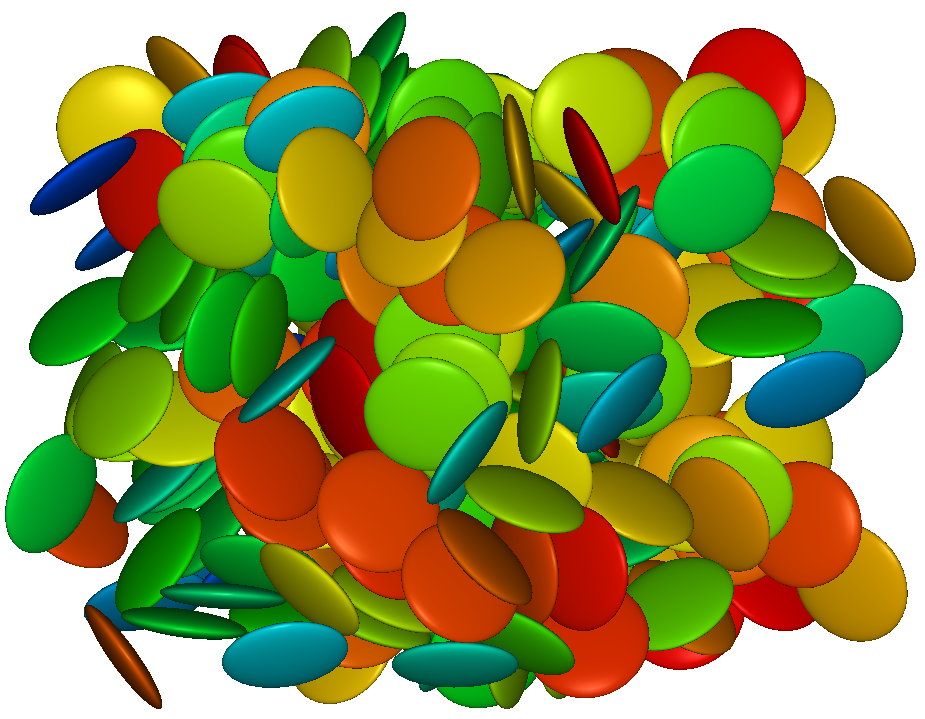
\includegraphics[width=.3\linewidth]{images/isotropic.png}
 \caption{Isotropic phase. Images are from bulk simulations at different temperatures and are visualized with the software QMGA \cite{qmga}.}
 \label{fig:isotropic}
\end{figure}

As the name suggests this phase is characterized by the isotropy of the system, that is, there is no orientational correlation between the molecules. There are however, as opposed to an ideal gas, short range spatial correlations as found in any other fluid.
\subsubsection{Nematic Phase}
\begin{figure}[H]
 \centering
 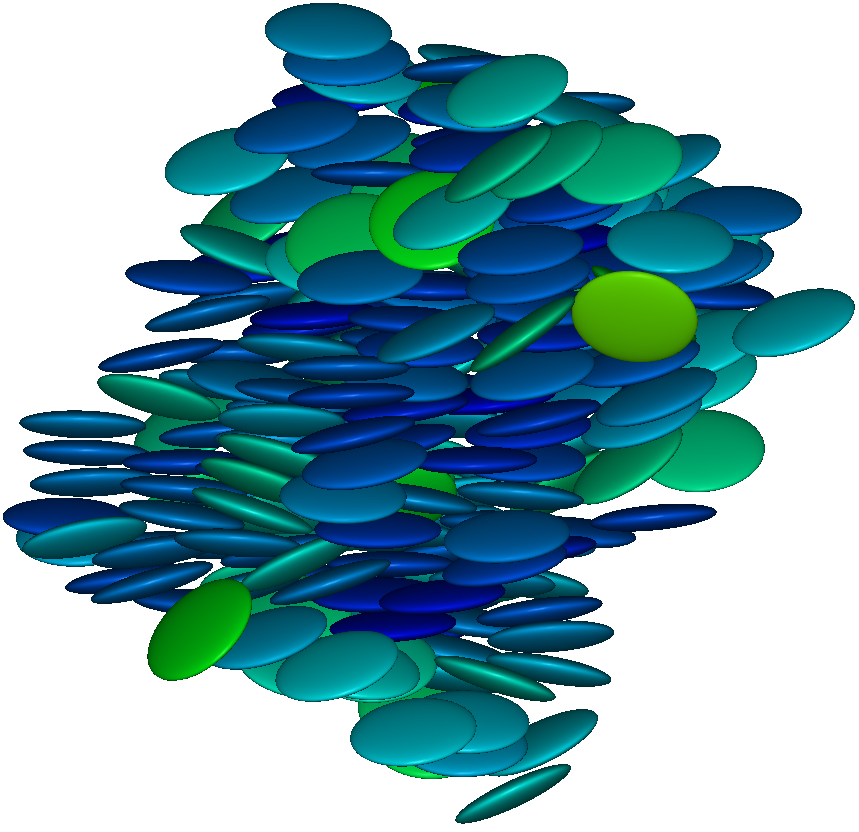
\includegraphics[width=.3\linewidth]{images/nematic.png}
 \caption{Nematic phase}
 \label{fig:nematic}
\end{figure}
The characteristic property of the nematic phase is that while there are no long range spatial correlations between the molecules, there is a distinct orientational preference, i.e. the particles are mostly aligned along a specific direction, represented with a vector called the director $\hat{\mathbf{n}}$. The system remains invariant under rotations around $\hat{\mathbf{n}}$. The phase therefore possesses a $D_{\infty h}$ symmetry.
\subsubsection{Columnar Phase}
\begin{figure}[H]
 \centering
 \subfigure[Seen from the side\label{fig:columnarside}]
   {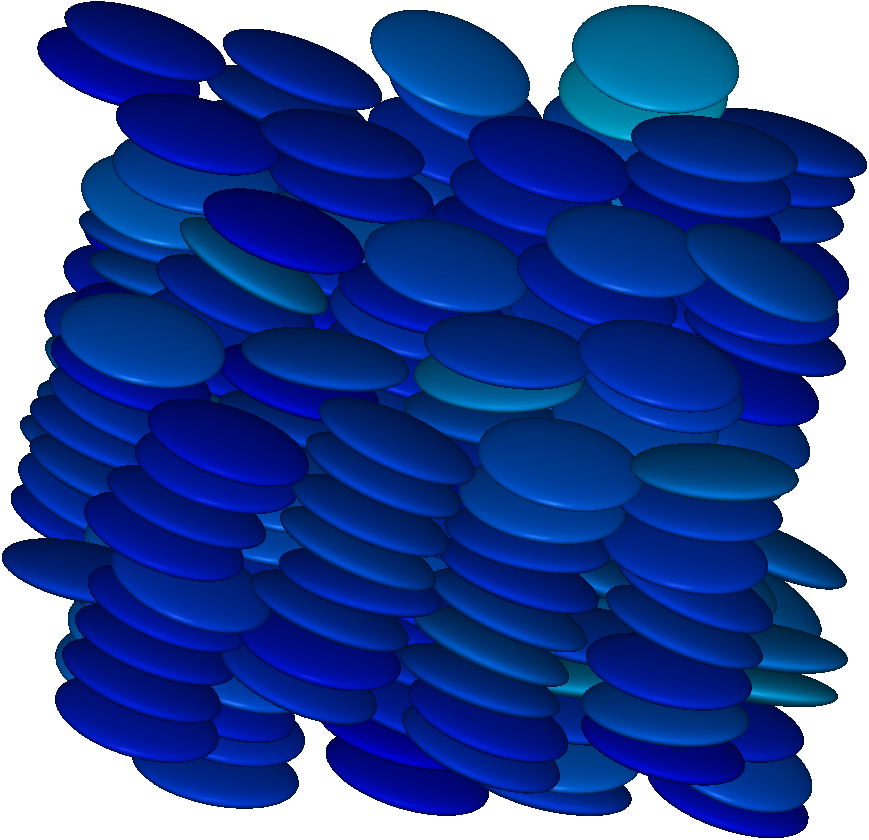
\includegraphics[width=0.3\textwidth]{images/columnar.png}}
\subfigure[Seen from above\label{fig:columnarabove}]
   {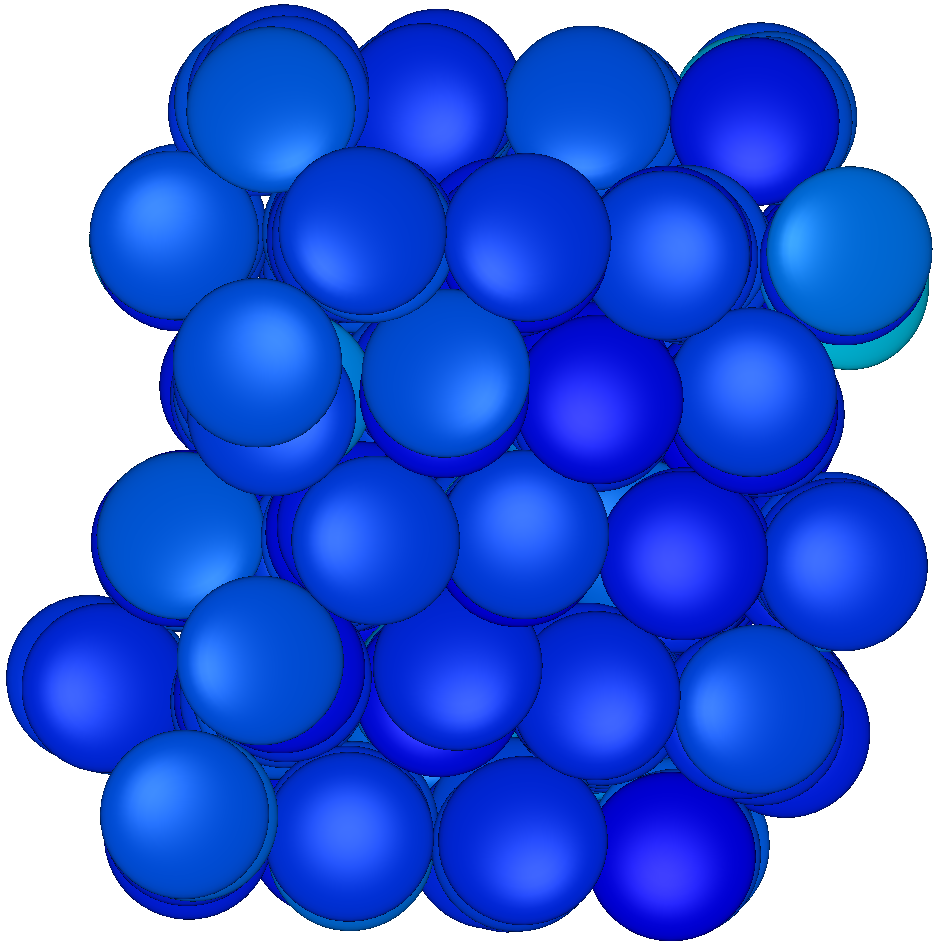
\includegraphics[width=0.3\textwidth]{images/columnarabove.png}}
 \caption{Columnar phase}
\end{figure}

At lower temperatures, molecular interactions favor an arrangement where the molecules stack on top of each other, and thus long columns in one direction emerge. The columns arrange themselves in a hexagonal lattice, since the highest-density configuration for circles in 2-D planes is the hexagonal packing arrangement \cite{chang2010simple}. 
The system is liquid in one dimension, along the columnar axis, and solid in the other two.
This phase possesses a $D_{6 h}$ symmetry.
\subsubsection{Crystal Phase}
\begin{figure}[H]
 \centering
 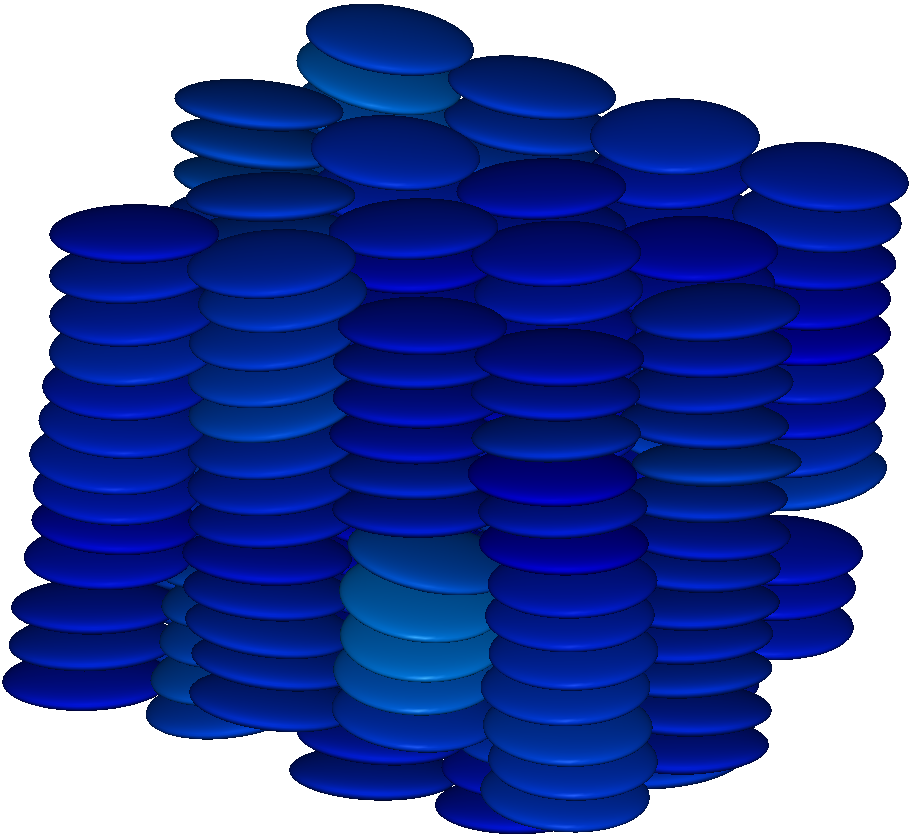
\includegraphics[width=.3\linewidth]{images/crystal.png}
 \caption{Crystal phase}
 \label{fig:Crystal phase}
\end{figure}
Upon further cooling, the individual columns solidify, creating a body-centred orthorhombic crystal phase.

\subsubsection{Confined Phases}
\label{subsubsec:confinedphases}
By restricting the geometry of the liquid crystal system one can favor certain phases, shifting the phase diagram, and create new configurations entirely \cite{zhang2015columnar,sentker2018quantized}.
A confining wall will induce a preferential alignment of the liquid crystal molecules at its surface, because of physical and chemical interactions. We call this preferential alignment `anchoring'.
In particular, by confining the system to a cylindrical shape and enforcing a circular edge-on anchoring of the particles to the outer wall, i.e, by favoring an alignment of the molecules near the wall perpendicular to both the radial position and the cylindrical axis, one can observe the quantized appearance of concentric columnar rings. Starting from the wall, the annular layers propagate inward layer-by-layer discretely. 
\begin{figure}[H]
 \centering
 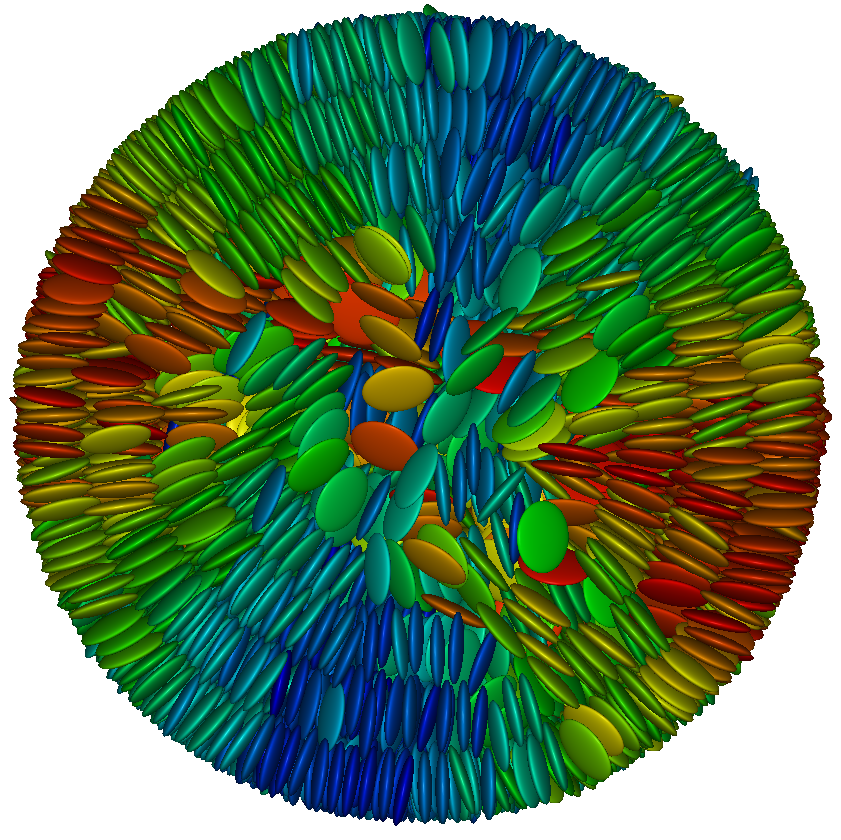
\includegraphics[width=.3\linewidth]{images/confined.png}
 \caption{Concentric columnar rings arising due to the cylindrical confinement. \cite{sentker2018quantized}}
 \label{fig:pore}
\end{figure}


\subsection{Order parameters}
\label{subsec:orderparameters}
The goal of this subsection is to define a suitable order parameter with which we can describe the phase transitions of the given liquid-crystal system.

\subsubsection{Nematic order parameter}
We can study many physical properties of a given material by their reaction to a (small) perturbation such as an electric or magnetic field. Our goal is to define an orientational order parameter. Therefore it is sensible to consider the orientation of both the perturbation and the reaction. Given a perturbation $P_\beta$, we can write the reaction $R_\alpha$ as
\begin{align*} 
    R_\alpha = {R_0}_\alpha + \displaystyle\sum_\beta\chi_{\alpha\beta} P_\beta + \displaystyle\sum_{\beta,\chi}\chi_{\alpha\beta\gamma} P_\beta P_\gamma + ...
\end{align*}
The physical properties of the material are encoded in the coefficients $\chi_{\alpha\beta},\, \chi_{\alpha\beta\gamma},\,...$. An orientational order parameter should describe how much the system deviates from an isotropic state. A good ansatz is thus to take the second order tensor $\chi_{\alpha\beta}$ and extract the isotropic part. This tensor can be represented by a $3\!\times\!3$ matrix, which we shall denote by $\chi$.

Because of the $D_{\infty h}$ symmetry of the discotic liquid crystal molecule, the matrix takes the form
\begin{align}
   \chi = \begin{pmatrix}
    \chi_\perp&0&0\\
    0&\chi_\perp&0\\
    0&0&\chi_\parallel
    \end{pmatrix}
\end{align}
in the coordinate system where the orientation of the LC molecule is given by $\hat{\mathbf{e}}=(0,0,1)^T$.
In any other reference frame the matrix is then given by $\chi' \equiv R\chi R^{-1}$, where $R$ is the rotation matrix to that reference frame. Since we wish to define a parameter that vanishes when the material is completely isotropic and is 1 when it is fully aligned, we need to extract the isotropic component of the matrix, given by  $\frac{\mathrm{tr}(\chi)}{3}\id$ . Therefore we find that  $\chi' - \frac{\mathrm{tr}(\chi)}{3}\id$ is the anisotropic part of the tensor $\chi'$. Let's consider explicity $\chi' - \frac{\mathrm{tr}(\chi)}{3}\id$ :
\begin{align*}
    \chi' - \frac{\mathrm{tr}(\chi)}{3}\id &= R\chi R^{-1} - \frac{\mathrm{tr}(\chi)}{3}\id \\
                                           &= R (\chi - \frac{\mathrm{tr}(\chi)}{3}\id) R^{-1} \\ 
                                           &= R \left(\frac{1}{3}\left(3  
    \begin{pmatrix}
    \chi_\perp&0&0\\
    0&\chi_\perp&0\\
    0&0&\chi_\parallel
    \end{pmatrix}
    -
    \begin{pmatrix}
    2\chi_\perp+\chi_\parallel&0&0\\
    0&2\chi_\perp+\chi_\parallel&0\\
    0&0&2\chi_\perp+\chi_\parallel
    \end{pmatrix}\right)\right)R^{-1}\\
    &= R \left(\frac{1}{3} 
    \begin{pmatrix}
    \chi_\perp-\chi_\parallel&0&0\\
    0&\chi_\perp-\chi_\parallel&0\\
    0&0&2(\chi_\perp-\chi_\parallel)
    \end{pmatrix}
    \right)R^{-1} \\
    &=  \Delta \chi \, R \left( 
    \begin{pmatrix}
    0&0&0\\
    0&0&0\\
    0&0&1
    \end{pmatrix}
    -\frac{1}{3}
    \begin{pmatrix}
    1&0&0\\
    0&1&0\\
    0&0&1
    \end{pmatrix} \right)
    R^{-1},  \qquad \text{where }\Delta \chi= \chi_\parallel - \chi_\perp \\ 
    &= \Delta \chi (R (\hat{\mathbf{e}} \otimes \hat{\mathbf{e}} - \frac{1}{3} \id)R^{-1}) \\
    &= \Delta \chi (R (\hat{\mathbf{e}}\otimes \hat{\mathbf{e}}) R^{-1} - \frac{1}{3} \id) \\
    &= \Delta \chi (\hat{\mathbf{e}'}\otimes \hat{\mathbf{e'}} - \frac{1}{3} \id).
\end{align*}
We can therefore define the nematic order parameter is the average normalized anisotropy over the entire system $Q \equiv \langle \frac{3}{2}(\hat{\mathbf{e}'}\otimes \hat{\mathbf{e'}} - \frac{1}{3} \id )\rangle$. The scalar order parameter $S$ is defined as the largest eigenvalue\footnote{This is well-defined, since $Q$ is a symmetric matrix. By the principal axis theorem $Q$ has three real eigenvalues, in particular a largest eigenvalue.} of $Q$ and the director $\hat{\mathbf{n}}$  as the corresponding eigenvector.
This definition allows some insight into the nature of the scalar order parameter. Keeping the same notation we have
\begin{align*}
    S &= S \hat{\mathbf{n}}^T \hat{\mathbf{n}}    \\
      &= \hat{\mathbf{n}}^T Q \hat{\mathbf{n}}\\
      & = \langle \hat{\mathbf{n}}^T \frac{3}{2}  (\hat{\mathbf{e}}\otimes \hat{\mathbf{e}} - \frac{1}{3} \id) \hat{\mathbf{n}}\rangle\\
      &=  \frac{3}{2}  \langle (\hat{\mathbf{n}}^T \hat{\mathbf{e}}) (\hat{\mathbf{e}}^T \hat{\mathbf{n}}) - \frac{1}{3} \rangle\\
      &=   \langle \frac{1}{2}( 3\cos^2(\theta) - 1) \rangle \\
      &=   \langle P_2(\cos(\theta)) \rangle , \quad  P_2(x)= \frac{1}{2}( 3x^2 - 1).
\end{align*}
$P_2$ is the second Legendre polynomial, which corresponds to a quadrupolar symmetry, and the angle brackets indicate an ensemble average. We therefore conclude that the corresponding phase possesses a quadrupolar symmetry.
\subsubsection{Hexagonal order parameter}
In order to classify the columnar phase one needs to define an order parameter. The columnar phase is characterized by a 2D hexagonal lattice, therefore the hexagonal order parameter can be defined as
\begin{align}
    \Psi_6 = \left\langle \frac{1}{N} \displaystyle\sum^N_{i=1}  \frac{1}{|n_i|}\displaystyle\sum_{k,l\in n_i} \exp(6i \theta_{kl})  \right\rangle,
\end{align}
where $n_i$ denotes the particles in the immediate neighbourhood of the particle $i$. The angle $\theta_{kl}$ is calculated by taking the angle between the intermolecular vectors $\hat{\mathbf{r}}_{ik},\,\hat{\mathbf{r}}_{il}$ projected onto the plane orthogonal to the orientation vector $\hat{\mathbf{e}}_i$. The neighbourhood of the particle $i$ is defined as a thick annulus around $i$, whose thickness is $1.5\sigma_{\text{ff}}$ (see Section \ref{subsec:potentials}) and with an inner-ring radius of $0.5\sigma_{\text{ee}}$ and an outer-ring radius of $1.5\sigma_{\text{ee}}$. 
\subsubsection{Radial Distribution function}
Crystals are characterized by their light-scattering behaviour. In X-ray diffraction experiments, crystals exhibit strongly pronounced Bragg-peaks. The scattering spectrum is mathematically described by the structure factor
\begin{align}
    S(\mathbf{k}) = 1 + \int_V \exp(i \mathbf{k\cdot r})(g(\mathbf{r})-1) \text{d}\mathbf{r},
\end{align}
where $g(\mathbf{r})$ is called the pair correlation function\cite{allen1987computer}, defined as
\begin{align}
\label{eq:paircorrelation}
    g(\mathbf{r}) = \left\langle\frac{V}{N^2} \displaystyle\sum_i\displaystyle\sum_{i\neq j} \delta(\mathbf{r}-\mathbf{r}_{ij})\right\rangle,
\end{align}
where $\mathbf{r}_{ij}$ is the distance between two particles $i$ and $j$. In numerical applications, the Dirac delta distribution $\delta$ is replaced by a function which is non-zero in a small interval, thus essentially creating a histogram of pair separations in that range\footnote{Note that to normalize the histogram bins, one has to divide Eq. (\ref{eq:paircorrelation}) by the volume of the chosen interval}. The pair correlation function thus describes the probability of finding a particle at distance $\mathbf{r}$ from a reference particle. 

Since a system in an isotropic liquid phase has non-trivial short-term particle correlations the pair correlation function will not be constant, as opposed to an ideal gas for example. However, due to the isotropy of the system, it will be independent of the direction of the distance.

For a non-isotropic fluid that possesses a nematic phase, the pair correlation function will be different in the directions perpendicular to the director and the direction parallel to it. Based on Eq. (\ref{eq:paircorrelation}) one therefore can define two pair distribution functions as 
\begin{align}
    g_{\perp}(r) = \left\langle \frac{V}{N^2} \displaystyle\sum_i\displaystyle\sum_{i\neq j} \delta(r-r_{ij}^\perp)\theta\left(\sigma_{\text{ff}}-r_{ij}^\parallel\right) \right\rangle, \\
    g_{\parallel}(r) = \left\langle \frac{V}{N^2} \displaystyle\sum_i\displaystyle\sum_{i\neq j} \delta(r-r_{ij}^\parallel)\theta\left(\frac{\sigma_{\text{ee}}}{2}-r_{ij}^\perp\right)\right\rangle.
\end{align}
The components of the distance vector between two particles are
\begin{align*}
    \mathbf{r}_{ij}^\parallel &= \left(\mathbf{r}_{ij}\cdot\hat{\mathbf{e}}_i\right)\hat{\mathbf{e}}_i,\\
    \mathbf{r}_{ij}^\perp &= \mathbf{r}_{ij} - \mathbf{r}_{ij}^\parallel.
\end{align*}
The Heaviside function $\theta$ ensures a slicing of the space into sheets with thickness $2\sigma_{\text{ff}}$ and a column with diameter $\sigma_{\text{ee}}$ respectively.

Both the columnar and crystal phases exhibit sharp peaks in the perpendicular pair correlation at the positions of a hexagonal lattice, i.e., for $r_{\perp} \in \{ \sqrt{1+n+n^2}: n \in \mathbb{N}\}$. Since in the columnar phase, the particles in the columns behave like a one-dimensional liquid, the parallel pair correlation $g_\parallel$ will only show the short term correlations present in a liquid, whereas in the crystal phase it will exhibit the sharp peaks characteristic of crystals.

\subsubsection{Local order parameters}
In complex geometries, a global orientation of the particles may never occur and therefore investigating a local order parameter is necessary. In this section we will present a few order parameters with which we can investigate the local structure.
\paragraph {Local nematic order parameter}

The local nematic order parameter is calculated by averaging the nematic order at a neighbourhood $n_i$ of a particle $i$ over every particle.

\begin{align}
    S_L = \frac{1}{N}\displaystyle\sum_{i=1}^N  S(n_i)
\end{align}

The neighbourhood $n_i$ of the particle $i$ is taken to be a sphere of radius $\sigma_{ee}$ around it.

\iffalse
\subsubsection{Radial density}


$\rho(r) = (1/\pi r^2 h) (1/N) \sum_i \delta (r_i-r)$


\fi
\paragraph{Averaged bond order parameter}

When investigating the local molecular order, we use the spatially resolved average local bond order parameter $\overline{q}_l(i)$ as described by Lechner and Dellago \cite{lechner2008accurate}.





\section{Computational Methods}
\label{sec:compmethods}
Some physical systems are too complex to allow an analytical solution. In these cases computer simulations allow us to numerically study these systems and gain valuable insights. In this section we shall present a brief introduction to the theory behind the computational methods used in this work.

In statistical mechanics, one calculates an observable macroscopic property $A$ by integrating over the the phase space, i.e., the space of all possible configurations $\Gamma$
\begin{align}
\label{eq:observableexpectedvalue}
\langle A\rangle = \int \rho\left(\Gamma\right)  A\left(\Gamma\right) \mathrm{d}\Gamma
\end{align}
given the probability distribution $\rho$ of the system. Even when the solution for the probability distribution is known, the phase space usually has too high a dimensionality to exactly calculate the integral in Eq.(\ref{eq:observableexpectedvalue}). One method to solve this is to generate samples with the probability $\rho$ and calculate the average of $A$ over the samples, since for a sufficiently high number of samples
\begin{align*}
    \langle A\rangle_{\text{samples}}\equiv\frac{1}{N} \displaystyle\sum_{i=1}A(\Gamma_i) \approx \int \rho\left(\Gamma\right)  A\left(\Gamma\right) \mathrm{d}\Gamma =\langle A\rangle.
\end{align*}
To produce the samples one can use the Metropolis algorithm, which shall be presented in the next section.

\subsection{Metropolis Algorithm}
\label{subsec:metropolisalgorithm}
We begin by defining some important concepts in the derivation of the algorithm. Given a stochastic process, a Markov chain is a sequence of stochastic variables, with the property that the state of each stochastic process is only dependent on the state immediately preceding it.
Two states $\Gamma_n,\, \Gamma_m$ are linked by the probability $\pi_{mn}$, i.e. the probability that given $\Gamma_n$, the next outcome will be $\Gamma_m$. Given a probability distribution $\boldsymbol{\rho} = (\rho_1,...,\rho_n) $ for a state space $\{\Gamma_1,....\Gamma_n\}$ the probability that the next outcome is $\Gamma_m$ will be 
\begin{align}
\label{eq:markovmatrixmultiplication}
\rho_m' = \displaystyle\sum_i \pi_{mi} \rho_i.
\end{align}
Treating $\mathbb{\rho}$ as a vector, Eq. (\ref{eq:markovmatrixmultiplication}) becomes the well known multiplication of $\boldsymbol{\rho}$ by a matrix $\boldsymbol{\pi}$ which is called the transition matrix of the Markov process.
The time evolution of the system with a starting distribution $\boldsymbol{\rho}$ is given by the repeated multiplication of $\boldsymbol{\pi}$ with $\boldsymbol{\rho}$. An important result of the Markov chain theory is that (given some conditions on $\boldsymbol{\pi}$ \cite{grimmett2001probability,allen1987computer}) any starting distribution $\boldsymbol{\rho'}$ will converge to the limiting distribution $\boldsymbol{\rho}$, i.e. that $\displaystyle\lim_{n\to \infty} \boldsymbol{\pi}^n \boldsymbol{\rho'} = \boldsymbol{\rho}$. The limiting distribution then obviously satisfies 
\begin{align}
    \label{eq:limitingditributioneigenvectors}
    \boldsymbol{\rho} = \boldsymbol{\pi} \boldsymbol{\rho} \qquad \text{or} \qquad \rho_n = \displaystyle\sum_m \pi_{nm} \rho_m.
\end{align}
The goal is therefore to construct a matrix $\boldsymbol{\pi}$ such that the limiting distribution is the desired one. The method proposed by Hastings \cite{hastings1970monte} was to replace the eigenvalue equation (\ref{eq:limitingditributioneigenvectors}) by the stronger condition of detailed balance
\begin{align}
    \label{eq:detailedbalance}
    \pi_{mn} \rho_n = \pi_{nm} \rho_m.
\end{align}
Note that in this case there is no implied sum over the indices. For two different states $\rho_n,\rho_m$ a solution for the transition matrix is
\begin{align}
    \pi_{mn} =
    \begin{cases}
    \alpha_{mn} \frac{\rho_n}{\rho_m} , & \text{if } \rho_n<\rho_m\\
    \alpha_{mn} \phantom{\frac{\rho_n}{\rho_m}}, & \text{else}
     \end{cases}
\end{align}
for any symmetric stochastic matrix $\alpha_{mn}$. We still allow the state to remain the same by setting $\pi_{mm}=1-\sum_{m\neq n}\pi_{mn}$. The probability $\alpha_{mn}$ is called selection probability and represents the probability of generating the state $\Gamma_m$ given the state $\Gamma_n$, and  $\min\left\{1,\frac{\rho_n}{\rho_m}\right\}$ is called the acceptance probability, which determines whether the generated state $\Gamma_m$ is accepted or not. 
We are now able to write down the Metropolis algorithm in its most basic form.
\begin{enumerate}
    \item Initialize the system with an arbitrary state.
    \item \label{segno} Generate a random state according to the selection distribution $\alpha_{mn}$.
    \item Accept the new state with the accepting probability $\min\left\{1,\frac{\rho_n}{\rho_m}\right\}$.
    \item Go to \ref{segno}.
\end{enumerate}



\subsection{Isothermal-Isobaric Monte Carlo}
\label{subsubsec:isothermalisobaricMC}
The Metropolis algorithm can be applied to any number of ensembles to calculate averages. In 1968, Woods \cite{wood1968monte} first applied this method for an isothermal-isobaric ensemble, a system with a constant pressure $P$, temperature $T$ and number of particles $N$. The probability distribution for this system is proportional to
\begin{align}
    \rho \propto  V^N \exp(- \beta (PV+ \mathcal{H})).
\end{align}
From this we see that the ratio of the probabilities of two states is given by
\begin{align}
    \frac{\rho_n}{\rho_m} &= \frac{V_{n}^N\exp(-\beta PV_n+\mathcal{H}_n))}{V_{m}^N\exp(-\beta(PV_m+\mathcal{H}_m))}\\
                          &= \exp(-\beta (P\Delta V_{nm} + \Delta\mathcal{V}_{nm})+N\log(V_n/V_m)),
\end{align}
where  $\Delta V_{nm}$ denotes the difference in volume between the two states and $\Delta\mathcal{V}_{nm}$ the potential difference.

We generate a new step by displacing a particle randomly and changing the volume according to
\begin{align}
    \mathbf{r}_m &= \mathbf{r}_n+ \delta r (2\mathbf{x}-1),\\
    \hat{\mathbf{e}}_m &= \frac{\hat{\mathbf{e}}_n+ \delta e\hat{\mathbf{x}}}{||\hat{\mathbf{e}}_n+ \delta e\hat{\mathbf{x}}||} ,\\
    V_m &= V_n + \delta V (2x-1),
\end{align}
where $\mathbf{x}$ denotes a vector whose components are uniformly distributed random numbers on $[0,1]$, $x$ is a uniform random number on $[0,1]$, $\hat{\mathbf{x}}$ is a vector uniformly distributed on a unit sphere and $\delta r,\,\delta e ,\, \delta V$ are parameters that dictate the maximum change in position and volume respectively.


\subsection{Parallel Tempering}
\label{subsubsec:paralleltemp}
While the convergence of the Metropolis algorithm is guaranteed as the running time approaches infinity, the simulated system can become stuck in local potential wells. One possible solution to this problem is to use the method of parallel tempering. The main idea of this method is to simulate $M$ copies of the same system at different temperatures $T_1 < ... < T_M$. A system with a higher temperature will generally sample a larger region of the phase space, whereas a low temperature system will sample a smaller region more finely. By allowing these systems to swap configurations every so often, we can achieve a more representative collection of samples of a low temperature system. There is a way to regulate these swaps in a way such that the detailed balance condition (\ref{eq:detailedbalance}) is preserved.

We can view the $M$ simulations as part of one big ensemble. Without any interaction between the systems, they are statistically independent. The probability distribution function for the collection of states $\{\Gamma^{T_1}_1,...,\Gamma^{T_M}_M\}$ at the respective temperature is therefore given by
\begin{align}
    \rho = \displaystyle\prod_{i=1}^M \rho^{T_i}_i.
\end{align}
To satisfy detailed balance the swapping probability $\pi_{ij}$ between two systems $\Gamma_i^{T_i},\,\Gamma_j^{T_j}$ must be
\begin{align}
    \pi_{ij} \rho^{T_1}_1...\rho^{T_i}_i...\rho^{T_j}_j...\rho^{T_M}_M &= \pi_{ji} \rho^{T_1}_1...\rho^{T_i}_j...\rho^{T_j}_i...\rho^{T_M}_M \\
    \pi_{ij} &= \pi_{ji} \frac{\rho^{T_i}_j\rho^{T_j}_i}{\rho^{T_i}_i\rho^{T_j}_j}.
\end{align}
We carry out the discussed algorithm in each of the steps individually, but in addition we add an extra step of swapping two systems $\Gamma_{T_i},\, \Gamma_{T_j}$ with the probability
\begin{align}
    \min\left\lbrack1, \exp(-(\beta_i-\beta_j)(\mathcal{V}_i-\mathcal{V}_j)\right\rbrack.
\end{align}
In a similar fashion to Sec. \ref{subsec:metropolisalgorithm} this satisfies detailed balance, and therefore converges to the desired probabilities.




\subsection{Potentials}
\label{subsec:potentials}
To perform Monte Carlo simulations of our liquid system we need to define potentials for the intermolecular interaction. The actual electromagnetic potential is far too complex to calculate due to the number and complexity of the molecules. Fortunately, we can obtain realistic results and a large number of mesophases by taking an effective model potential that reflects the symmetries of the molecules. In the following we shall present and discuss the choice for these models.
\subsubsection{Improved Gay-Berne Model}
One of the first single-site potentials to represent aspherical particles was introduced by Berne and Pechukas\cite{gay1981modification}. It is obtained by computing the overlap integral of two identical, ellipsoidal Gaussians of arbitrary relative orientation
\begin{align}
 \exp\left\lbrack-\frac{x^2+y^2}{\sigma_{\text{ee}}^2}-\frac{z^2}{\sigma_{\text{ff}}^2}\right\rbrack.
\end{align}
Taking $\mathbf{\hat{e}}_1,\mathbf{\hat{e}}_2$ to be unit vectors, specifying the orientation of the two Gaussians, $\mathbf{r}$ as the distance between their centers, $r= ||\mathbf{r}||$ and $\mathbf{\hat{r}} = \frac{\mathbf{r}}{r}$, the expression for the integral is
\begin{align}
S(\mathbf{\hat{e}}_1,\mathbf{\hat{e}}_2,\mathbf{r}) = \epsilon_1(\mathbf{\hat{e}}_1,\mathbf{\hat{e}}_2)\cdot \exp\left\lbrack - \frac{r^2}{\sigma^2(\mathbf{\hat{e}}_1,\mathbf{\hat{e}}_2,\mathbf{\hat{r}})}\right\rbrack,
\end{align}
where
\begin{align}
\label{eq:strengthparameter}
    \epsilon_1(\mathbf{\hat{e}}_1,\mathbf{\hat{e}}_2) = \epsilon_0(1-\chi^2(\mathbf{\hat{e}}_1\cdot\mathbf{\hat{e}}_2))
\end{align}
is called the strength parameter, and
\begin{align} 
\label{eq:rangeparameter}
\sigma(\mathbf{\hat{e}}_1,\mathbf{\hat{e}}_2,\mathbf{r})&= \sigma_0 \Bigg\{ 1- \frac{\chi}{2}\left\lbrack \frac{(\mathbf{\hat{r}}\cdot\mathbf{\hat{e}}_1+\mathbf{\hat{r}}\cdot\mathbf{\hat{e}}_2)^2}{1+\chi(\mathbf{\hat{e}}_1\cdot\mathbf{\hat{e}}_2)}+\frac{(\mathbf{\hat{r}}\cdot\mathbf{\hat{e}}_1-\mathbf{\hat{r}}\cdot\mathbf{\hat{e}}_2)^2}{1-\chi(\mathbf{\hat{e}}_1\cdot\mathbf{\hat{e}}_2)}\right\rbrack\Bigg\}^{-\frac{1}{2}}
\end{align}
is called the range parameter. The coefficient $\chi$ is defined as
\begin{align}
\label{eq:anisotropyparameter}
    \chi &= \frac{\sigma_\text{ff}^2-\sigma_\text{ee}^2}{\sigma_\text{ff}^2+\sigma_\text{ee}^2}
\end{align}
and is called the anisotropy parameter. The overlap potential is then obtained by modifying the Lennard-Jones potential:
\begin{align}
    \label{eq:overlappotential}
    V(\mathbf{\hat{e}}_1,\mathbf{\hat{e}}_2,\mathbf{r}) &= 4\epsilon(\mathbf{\hat{e}}_1,\mathbf{\hat{e}}_2,\mathbf{r}) \left\lbrack \left(\frac{\sigma(\mathbf{\hat{e}}_1,\mathbf{\hat{e}}_2,\mathbf{r})}{r}\right)^{12}-\left(\frac{\sigma(\mathbf{\hat{e}}_1,\mathbf{\hat{e}}_2,\mathbf{r})}{r}\right)^{6} \right\rbrack.
\end{align}
In many ways, this potential is unrealistic \cite{gay1981modification} and therefore was modified in two ways by Gay and Berne  and later by Bates and Luckhurst \cite{bates1996computer} further to better reflect the properties and behaviour of discotic molecules. 
\begin{enumerate}
    \item We modify \begin{align}
       \frac{\sigma(\mathbf{\hat{e}}_1,\mathbf{\hat{e}}_2,\mathbf{r})}{r} \to \frac{1}{r-\sigma(\mathbf{\hat{e}}_1,\mathbf{\hat{e}}_2)+1}.
    \end{align}
    In this way the width of the potential well between two particles is independent of their relative orientations.
    \item We set 
    \begin{align}
        \epsilon(\mathbf{\hat{e}}_1,\mathbf{\hat{e}}_2) = \epsilon_1^\nu(\mathbf{\hat{e}}_1,\mathbf{\hat{e}}_2) \epsilon_2^\mu(\mathbf{\hat{e}}_1,\mathbf{\hat{e}}_2,\mathbf{\hat{r}}),
    \end{align}
    where $\epsilon_1(\mathbf{\hat{e}}_1,\mathbf{\hat{e}}_2)$ is the original strength parameter defined in Eq. (\ref{eq:strengthparameter}) and $\epsilon_2(\mathbf{\hat{e}}_1,\mathbf{\hat{e}}_2,\mathbf{\hat{r}})$ defined as
    \begin{align}
        \epsilon_2(\mathbf{\hat{e}}_1,\mathbf{\hat{e}}_2,\mathbf{\hat{r}})= 1-\frac{\chi'}{2}\left\lbrack\frac{(\mathbf{\hat{r}}\cdot\mathbf{\hat{e}}_1+\mathbf{\hat{r}}\cdot\mathbf{\hat{e}}_2)^2}{1+\chi'\mathbf{\hat{e}}_1\cdot\mathbf{\hat{e}}_2}+\frac{(\mathbf{\hat{r}}\cdot\mathbf{\hat{e}}_1-\mathbf{\hat{r}}\cdot\mathbf{\hat{e}}_2)^2}{1-\chi'\mathbf{\hat{e}}_1\cdot\mathbf{\hat{e}}_2}\right\rbrack
    \end{align}
    to adjust the side-by-side and face-to-face well-depths. Taking $\epsilon_{\text{ss}}$ to be the value of the strength parameter for a side-by-side configuration and $\epsilon_{\text{ff}}$ to be the value of the strength parameter for a face-to-face configuration, $\chi'$ is defined to be
    \begin{align}
        \chi'=  \frac{(\epsilon_{\text{ss}}/\epsilon_{\text{ff}})^\frac{1}{\mu}-1}{(\epsilon_{\text{ss}}/\epsilon_{\text{ff}})^\frac{1}{\mu}+1}.    
    \end{align}
    For discotics setting $\mu=1$, $\nu=2$ gives the desired behaviour \cite{gay1981modification}.
    \item For small values of $r$ the potential still shows unrealistic behaviour \cite{bates1996computer}. If two particles approach each other face to face, the potential does not tend to infinity at $r \to 0$, but rather at $r \to \sigma_{\text{ee}}-\sigma_{\text{ff}}$ which in our case is negative and therefore is unphysical. To correct this, Bates and Luckhurst proposed the modification
    \begin{align}
        \frac{1}{r-\sigma(\mathbf{\hat{e}}_1,\mathbf{\hat{e}}_2)+1} \to \frac{\sigma_{\text{ff}}}{r-\sigma(\mathbf{\hat{e}}_1,\mathbf{\hat{e}}_2,\mathbf{r})+\sigma_\text{ff}}.
    \end{align}
    The modified Gay-Bern potential was named {GBDII} and is the model we use in this work. 
\end{enumerate}
In its entirety the potential becomes
\begin{align}
    \label{eq:GBDII}
    V(\mathbf{\hat{e}}_1,\mathbf{\hat{e}}_2,\mathbf{r}) &= 4\epsilon(\mathbf{\hat{e}}_1,\mathbf{\hat{e}}_2,\mathbf{r}) \left\lbrack \left(\frac{\sigma_{\text{ff}}}{r-\sigma(\mathbf{\hat{e}}_1,\mathbf{\hat{e}}_2,\mathbf{r})+\sigma_{\text{ff}}}\right)^{12}-\left(\frac{\sigma_{\text{ff}}}{r-\sigma(\mathbf{\hat{e}}_1,\mathbf{\hat{e}}_2,\mathbf{r})+\sigma_{\text{ff}}}\right)^{6} \right\rbrack.
\end{align}

\subsubsection{Fluid-Wall Interaction}
\label{subsubsec:fluidwallinteraction}
Because we are interested in studying the liquid crystal confined by a cylindrical pore, we need another interaction potential.
A model for the interaction between the fluid and the wall can be obtained by integrating the Lennard-Jones potential on a semi-infinitely deep wall, to imitate a crystal with very densely packed spherical particles spanning over half of the three dimensional space. We thus get
\begin{align}
    \label{eq:wall_lennardjones}
    V_{\text{fw}}(\mathbf{r},\mathbf{\hat{e}})= \epsilon_{\text{fw}} \left\lbrack \frac{2}{15} \left(\frac{\sigma_\text{ff}}{d_w}\right)^9 -  \left(\frac{\sigma_\text{ff}}{d_w}\right)^3 \right\rbrack,
\end{align}
where $d_w = r_{\text{pore}}-|r|$ is the distance of the particle to the wall in cylindrical coordinates.
We implement the aforementioned circular edge-on anchoring (see Sec. \ref{subsubsec:confinedphases}) by scaling the attractive part of Eq. (\ref{eq:wall_lennardjones}) by the factor $ \left[(\mathbf{\hat{n}}_\text{w} \times \mathbf{\hat{e}} )\cdot \mathbf{\hat{z}}\right]^2$, where $\mathbf{\hat{n}}_\text{w}$ is the local normal to the wall. To take the shape anisotropy into account we modify 
\cite{sentker2018quantized,caprion2009discotic} the distance to the wall by the factor
\begin{align}
    \sigma_\text{w} (\mathbf{\hat{e}}) = \frac{\sigma_0}{2} \left\{\left\lbrack 1 - \frac{2 \chi_\text{w} (\mathbf{\hat{n}}_\text{w} \cdot \mathbf{\hat{e}} )^2)}{1+\chi_\text{w}} \right\rbrack -\frac{\sigma_\text{ff}}{\sigma_\text{ee}} \right\},
\end{align}
where $\chi_{\text{w}} = \frac{4\sigma_\text{ff}^2-\sigma_\text{ee}^2}{4\sigma_\text{ff}^2+\sigma_\text{ee}^2}$ is an adapted shape anisotropy $\chi$.
The potential then reads
\begin{align}
    \label{eq:wall_pot}
    V_{\text{fw}}(\mathbf{r},\mathbf{\hat{e}},\mathbf{\hat{n}})= \epsilon_{\text{fw}} \left\lbrack \frac{2}{15} \left(\frac{\sigma_\text{ff}}{d_w}- \sigma_\text{w} (\mathbf{\hat{e}}) \right)^9 - \left[(\mathbf{\hat{n}}_\text{w} \times \mathbf{\hat{e}} )\cdot \mathbf{\hat{z}}\right]^2  \left(\frac{\sigma_\text{ff}}{d_w- \sigma_\text{w} (\mathbf{\hat{e}}) }\right)^3 \right\rbrack.
\end{align}

\subsubsection{Fluid-Colloid Interaction}
In this work we want to study the effect of a colloidal particle on a system of discotic liquid crystals. A colloid is a type of mixture where the insoluble colloidal particles are suspended in the so-called dispersing phase and are significantly larger in size than the particles it is dispersed in.

We model the colloid with an unmovable spherical particle in the center of the system. The interaction of a liquid crystal particle with the colloid is described by a slightly modified Lennard-Jones potential. If $r$ is the distance between a fluid particle and the center of the colloid, we have 
\begin{align}
    V_{\text{fc}}(\mathbf{r},\mathbf{\hat{e}}) = 4\epsilon_{\text{fc}}\left\lbrack \left(\frac{\sigma_{\text{ff}}}{|r|-\lbrack r_{\text{c}}-\sigma_\text{w} (\mathbf{\hat{e}})\rbrack}\right)^{12} -  \left(\frac{\sigma_{\text{ff}}}{|r|-\lbrack r_{\text{c}}-\sigma_\text{w} (\mathbf{\hat{e}})\rbrack}\right)^6 \right\rbrack,
\end{align}
where $\epsilon_{\text{fc}}$ describes the strength of the potential, and $r_{\text{c}}$ is the radius of the colloid.
Again, the colloid interaction exhibits some orientational preference. To account for this we scale the attractive part of the potential by $g_{\text{orient}}(\mathbf{\hat{e}},\mathbf{\hat{n}})$
\begin{align}
\label{eq:orientation}
    g_\text{orient}(\mathbf{\hat{e}},\mathbf{\hat{n}}) = 
    \begin{cases}
     (\mathbf{\hat{e}}\cdot\mathbf{\hat{n}})^2 & \text{for face-on anchoring}\\
     (1-|\mathbf{\hat{e}}\cdot\mathbf{\hat{n}}|)^2 & \text{for edge-on anchoring.}
    \end{cases}
\end{align}
Since the colloid is spherical, the normal to the tangential surface at $\mathbf{r}$ is just the normalized distance vector $\mathbf{\hat{r}}$. The fluid-colloid potential thus becomes

\begin{align}
    V_{\text{fc}}(r) = 4\epsilon_{\text{fc}}\left\lbrack \left(\frac{\sigma_{\text{ff}}}{|r|-\lbrack r_{\text{c}}-\sigma_\text{w} (\mathbf{\hat{e}})\rbrack}\right)^{12} - g_\text{orient}(\mathbf{\hat{e}},\mathbf{\hat{r}}) \left(\frac{\sigma_{\text{ff}}}{|r|-\lbrack r_{\text{c}}-\sigma_\text{w} (\mathbf{\hat{e}})\rbrack}\right)^6 \right\rbrack.
\end{align}


\chapter{Implementation}
\label{chap:implementation}
\vspace{2cm}

\section{Reduced Units and Model Parameters}

Computationally, it is favourable to use reduced units in the simulations as they bring simplifications since we only have one type of particle. We set the fluid-fluid interaction parameter $\epsilon_0$ as well as the molecular diameter $\sigma_{\text{ee}}$ to one. From this the units of other measurable quantities change according to Table \ref{tab:reducedunits} \cite{allen1987computer }.

\begin{table}[H]
    \centering
    \begin{tabular}{|c|c|}
    \hline
        quantity  & unit dependency \\ \hline \hline
        length  &  $\sigma_{\text{ee}} = 1$ \\ \hline
        energy  & $\epsilon_0 =1 $ \\ \hline
        temperature & $T^{*} = k_{B}T/\epsilon_0$ \\ \hline
        pressure & $P^{*} = P\sigma_{\text{ee}}^3/\epsilon_0 $\\ \hline
        volume & $V^{*} = V/\sigma_{\text{ee}}^3 $\\ \hline
    \end{tabular}
    \caption{Reduced units of the used quantities}
    \label{tab:reducedunits}
\end{table}
With just reduced units however, the system is not fully parametrized. With the model potentials presented in Section \ref{subsec:potentials}, we set the remaining parameters as shown in Table \ref{tab:modelparam}.
\begin{table}[H]
    \centering
    \begin{tabular}{|c|c|}
    \hline
        parameter & value\\ \hline \hline
        $ \sigma_{\text{ff}}/\sigma_{\text{ee}} $ & $ 0.2$ \\ \hline
        $\epsilon_{\text{ff}}/\epsilon_{\text{ss}} $ & $ 0.2$\\ \hline
        $\epsilon_{\text{fw}} $ & $ 8$ \\ \hline
        $P^*$ & $ 50 $ \\ \hline
    \end{tabular}
    \caption{Parameters used in this work for the Gay-Bern potential (fluid-fluid interaction) and modified Lennard-Jones potential (fluid-colloid interaction) }
    \label{tab:modelparam}
\end{table}
The size anisotropy in the Gay-Berne potential is suitable to model an archetypal discotic molecule (HAT6) \cite{sentker2018quantized,caprion2003influence}. Following the work of Sentker, Zantop \textit{et al.} \cite{sentker2018quantized} we chose the fluid-wall interaction parameter to reproduce the quantized self-assembly of concentric rings in the confined system. The fluid-colloid interaction $\epsilon_{\text{cf}}$ was changed according to the specific system and the value is stated in the appropriate section.

\section{Simulations}

The simulations were performed with the aforementioned parallel tempering Monte Carlo algorithm.
There was an existing code for bulk simulations with periodic boundary conditions and cylindrically confined simulations with periodic boundary conditions in the $z$-direction, which I changed to include the colloid interactions. 

To produce an equilibrated system, the system performs $3\cdot10^5$ steps according to the isothermal-isobaric Monte Carlo algorithm delineated in Sec. \ref{subsubsec:isothermalisobaricMC} for $N_T$ systems with different temperatures. 
After each step, a system swap is then attempted according to Sec.\ref{subsubsec:paralleltemp} for two random systems with adjacent temperatures. After the equilibration steps, the system will perform $5\cdot10^4$ additional steps, logging the system size, positions and orientations at every temperature every 500 steps to produce 100 ensemble samples. To reduce correlations between samples the simulations were repeated and the relevant observables were computed with all samples from the respective systems. 

To compute the in Sec.\ref{subsec:orderparameters} mentioned order parameters with the samples I wrote programs in \texttt{Python}.


\chapter{Results}
\label{chap:results}
\vspace{1cm}

\section{Confined System}
\label{sec:confinedsystem}
\subsection{Edge-On Anchoring}

In Figure \ref{fig:confsnapshots} we can see a cross section of the confined system for various sizes of colloids. We can see that the imposed structure of the colloid is compatible with the imposed structure of the pore.
\begin{figure}[H]
 \centering
 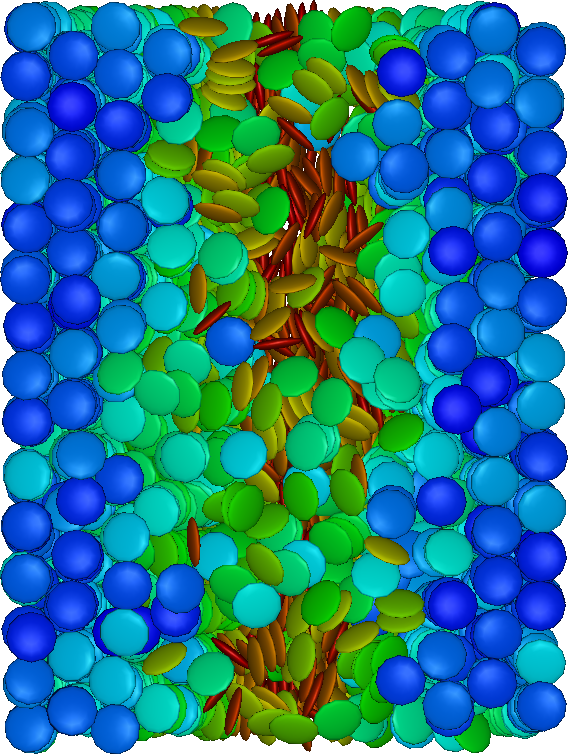
\includegraphics[width=.2\linewidth]{images/ceo_W8C8_D0.png}
 \qquad
 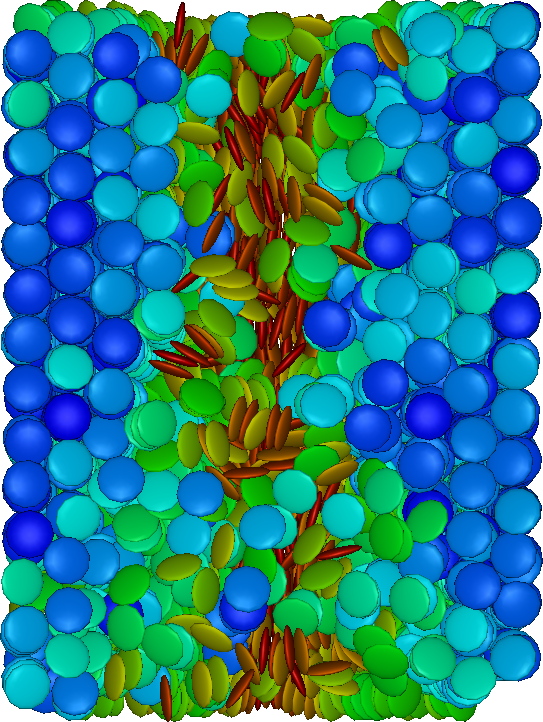
\includegraphics[width=.2\linewidth]{images/ceo_W8C8_D3.png}
 \qquad
 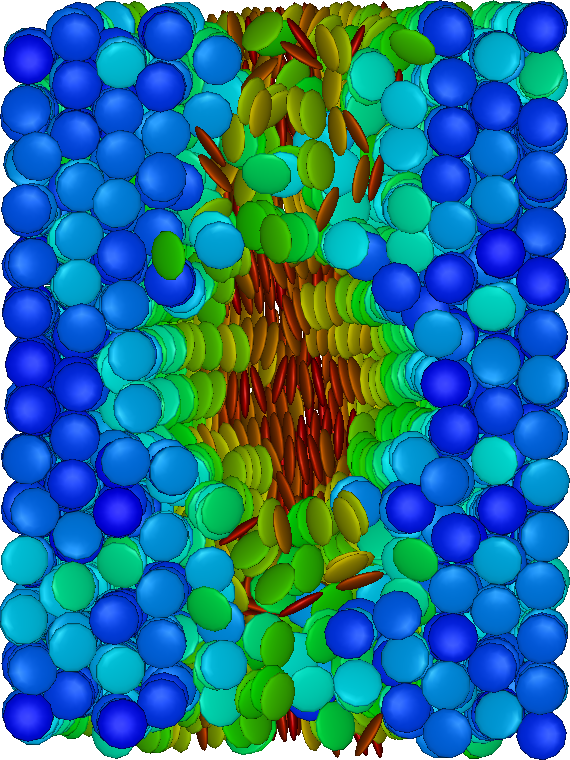
\includegraphics[width=.2\linewidth]{images/ceo_W8C8_D6.png}
 \qquad
 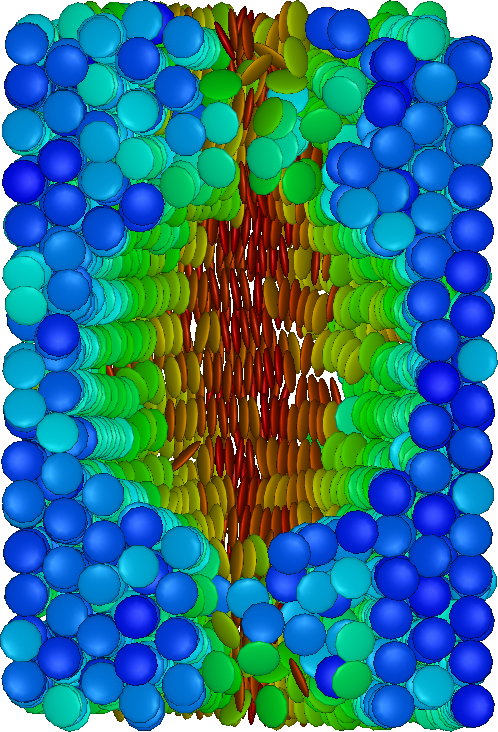
\includegraphics[width=.2\linewidth]{images/ceo_W8C8_D9.png}
 \caption{Cross sectional snapshots of the confined discotic liquid crystal system at $P^* = 50$, $T^* = 5.0$ with no colloid (far left), and with colloids of diameter $D^* \in \{3,6,9\} $. The pore diameter is $11.25\sigma_{ee}$.}
 \label{fig:confsnapshots}
\end{figure}
We can study the behaviour of the system through the various order parameters. 
Figure \ref{fig:ceoC8nemloc} shows the dependence of the local nematic order parameter on the temperature. We can see a quantized assembly of rings as found by Arne happening for every size of colloids. However, we can also see that as the colloidal size increases, the transitions happen at higher temperature and that the meta-stable plateaus appearing for smaller colloids become more sloped and the transitions become more soft. 


\begin{figure}[H]
    \centering
	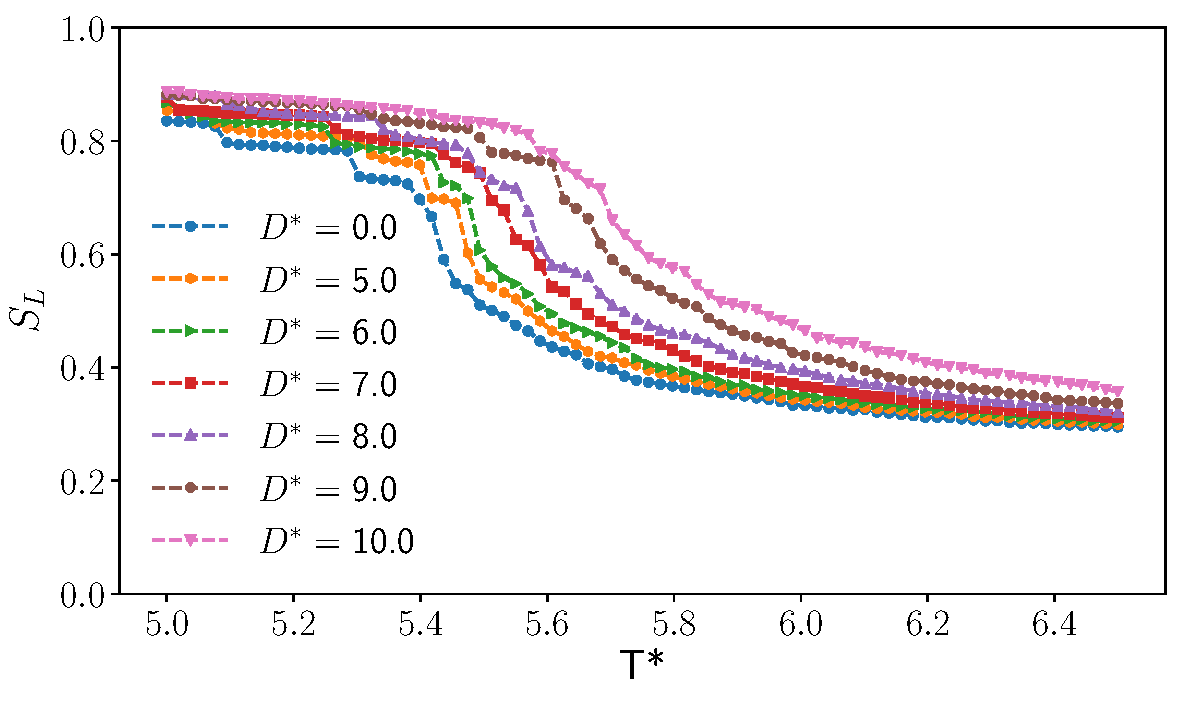
\includegraphics[width=0.8\linewidth]{plots/ceo_W8C8_nemloc.pdf}
	\caption{Dependence of the local nematic order parameter (left) and the hexagonal order parameter (right) on the temperature for confined systems with colloids of different size}
    \label{fig:ceoC8nemloc}
\end{figure}
To further study this appearance, we can look at the hexagonal order parameter which describes the columnar alignment of the rings, and the circular order parameter which describes the more general alignment along the concentric rings. 
Looking at the hexagonal order parameter we see more quantized transitions while the circular orientation
displays a similar behaviour to the local nematic order parameter which suggests that in the presence of a colloid, the circular concentric alignment of the molecules happens more continuously while the actual formation of columnar rings remainsdiscrete.  

\begin{figure}[H]
    \centering
	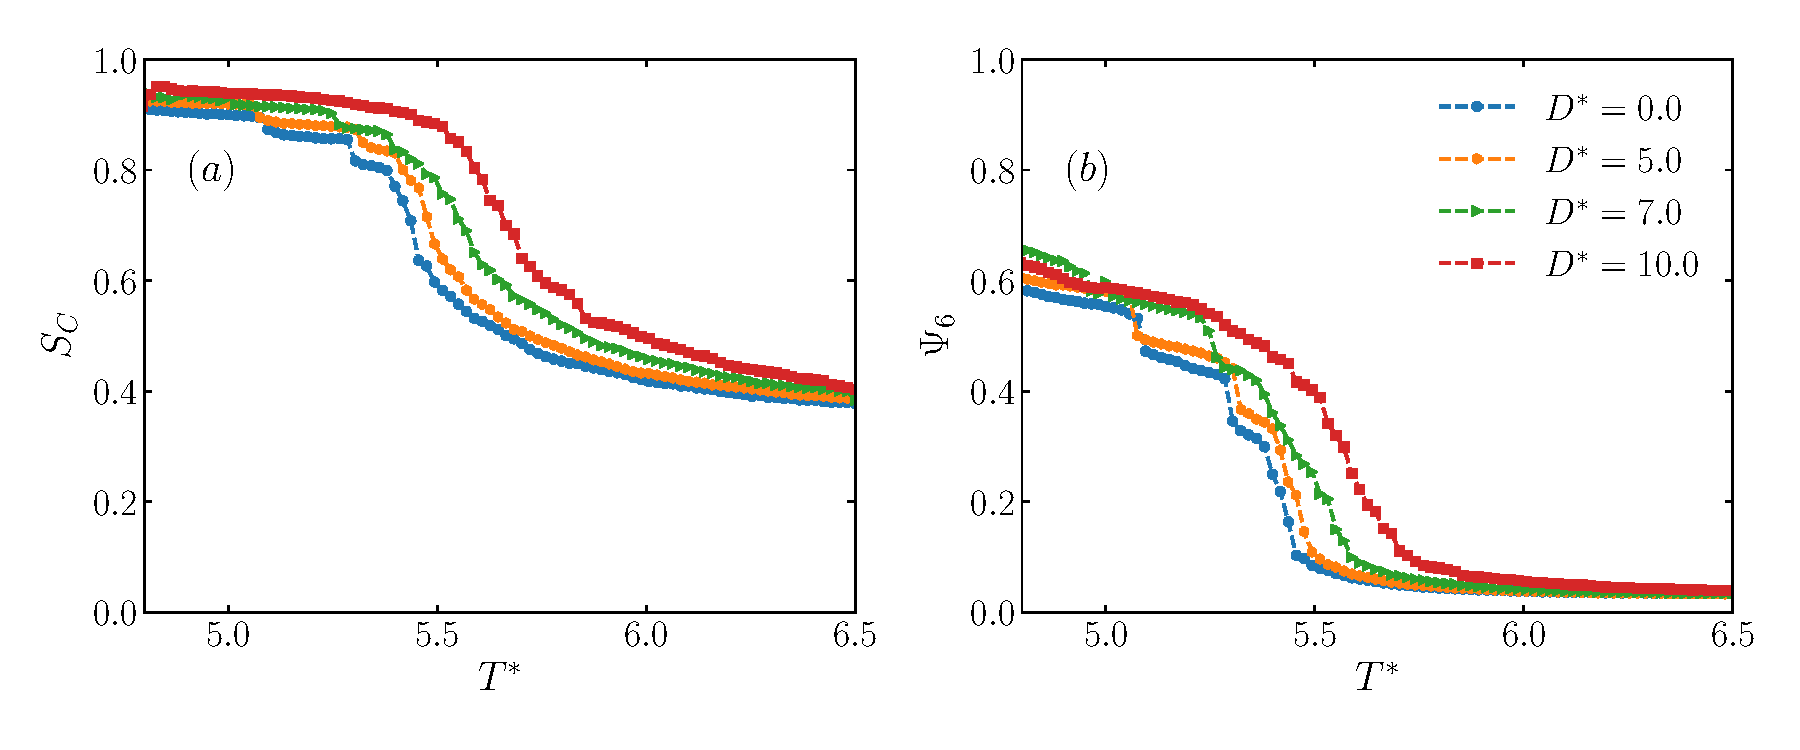
\includegraphics[width=\linewidth]{plots/ceo_W8C8_circhex.pdf}
	\caption{Dependence of the hexagonal order parameter and the circular order parameter on the temperature for confined systems with colloids of different size}
    \label{fig:ceoC8hex}
\end{figure}

If a confined system cools down even further (to $T^*< 4.5$), the inner rings start to break down, and a small domain of coaxially aligned molecules appears.
I have a feeling that the presence of a colloid would prevent that, which I would like to test in the near future. 


\label{sec:confinedsystem}
\subsection{Face-On Anchoring}
I did various simulations with various (often contradictory) results, and found out that for face-on anchoring, a high precision in the probed temperature range is very important, especially with strong colloid potentials. In the end I settled (for now) for a potential strength of $\epsilon_{\text{cf}}= 56\epsilon_{\text{ff}}$ since it produced fairly nice results.


Looking at the local nematic order parameter in function of the temperature, we see, that the nature of the transition does not change, which however is shifted towards colder temperatures, as the colloid grows in diameter.

\begin{figure}[H]
    \centering
	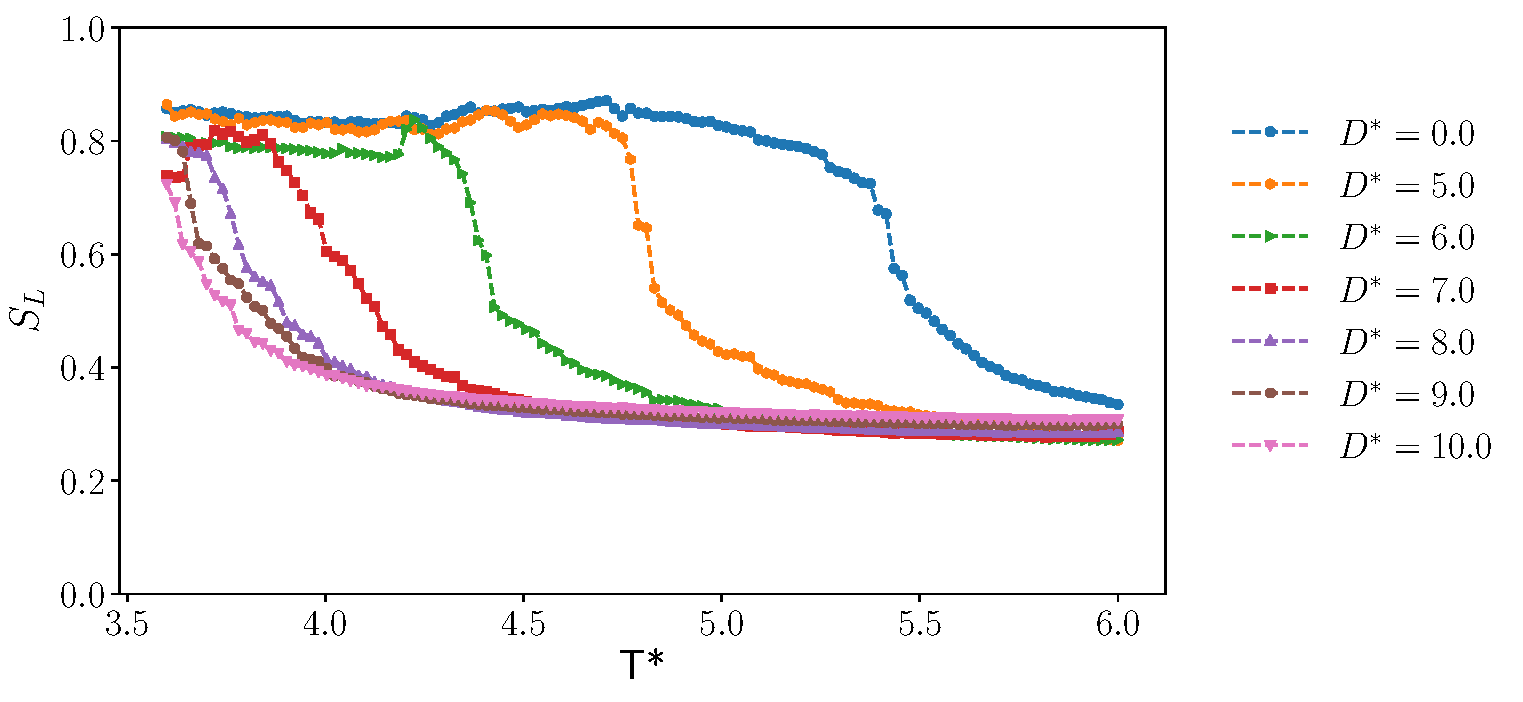
\includegraphics[width=\linewidth]{plots/cfo_W8C56_nemloc.pdf}
	\caption{Dependence of the local nematic order parameter and the hexagonal on the temperature for systems in bulk with colloids of different size}
    \label{fig:beoc32lochex}
\end{figure}
\begin{figure}[H]
    \centering
	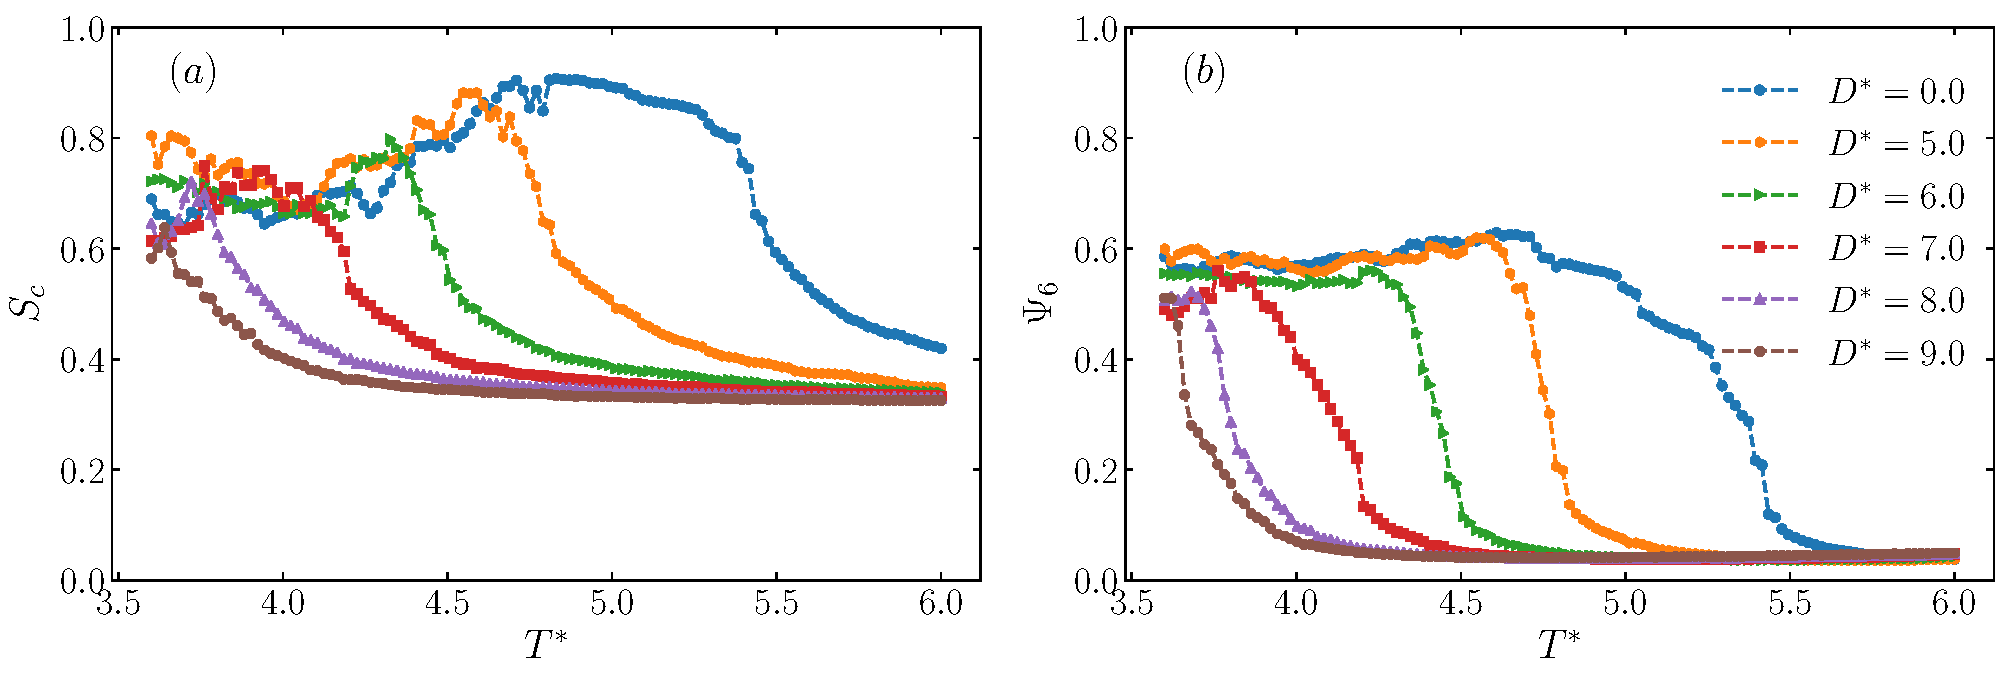
\includegraphics[width=\linewidth]{plots/cfo_W8C56_hexcirc.pdf}
	\caption{Dependence of the local nematic order parameter and the hexagonal on the temperature for systems in bulk with colloids of different size}
    \label{fig:cfohexcirc}
\end{figure}

Cooling the system even further down the inner rings break up/ never really form and the aforementioned domain of (generally) coaxially aligned particles, which can be seen by the drop in circular nematic order at lower temperatures in Figure \ref{fig:cfohexcirc}, whereas the local nematic order and hexagonal order stay fixed. If we look at the radial density, we can definitely see the formation of the concentric outer rings and can also "guess" the formation of the inner patch, in the way the become more blurred \footnote{I'm actually not really sure how to show this, since the alignment of that inner patch is not completely coaxial, but rather (sometimes very) sloped (see Fig, \ref{fig:cfosnapshots}. Also the distance between particles along the concentric planes remain $1\sigma_{\text{ee}}$ which is why probably the small peaks still appear at $r<3\sigma{\text{ee}}$ even if there are no actual rings.}.

\begin{figure}[H]
 \centering
 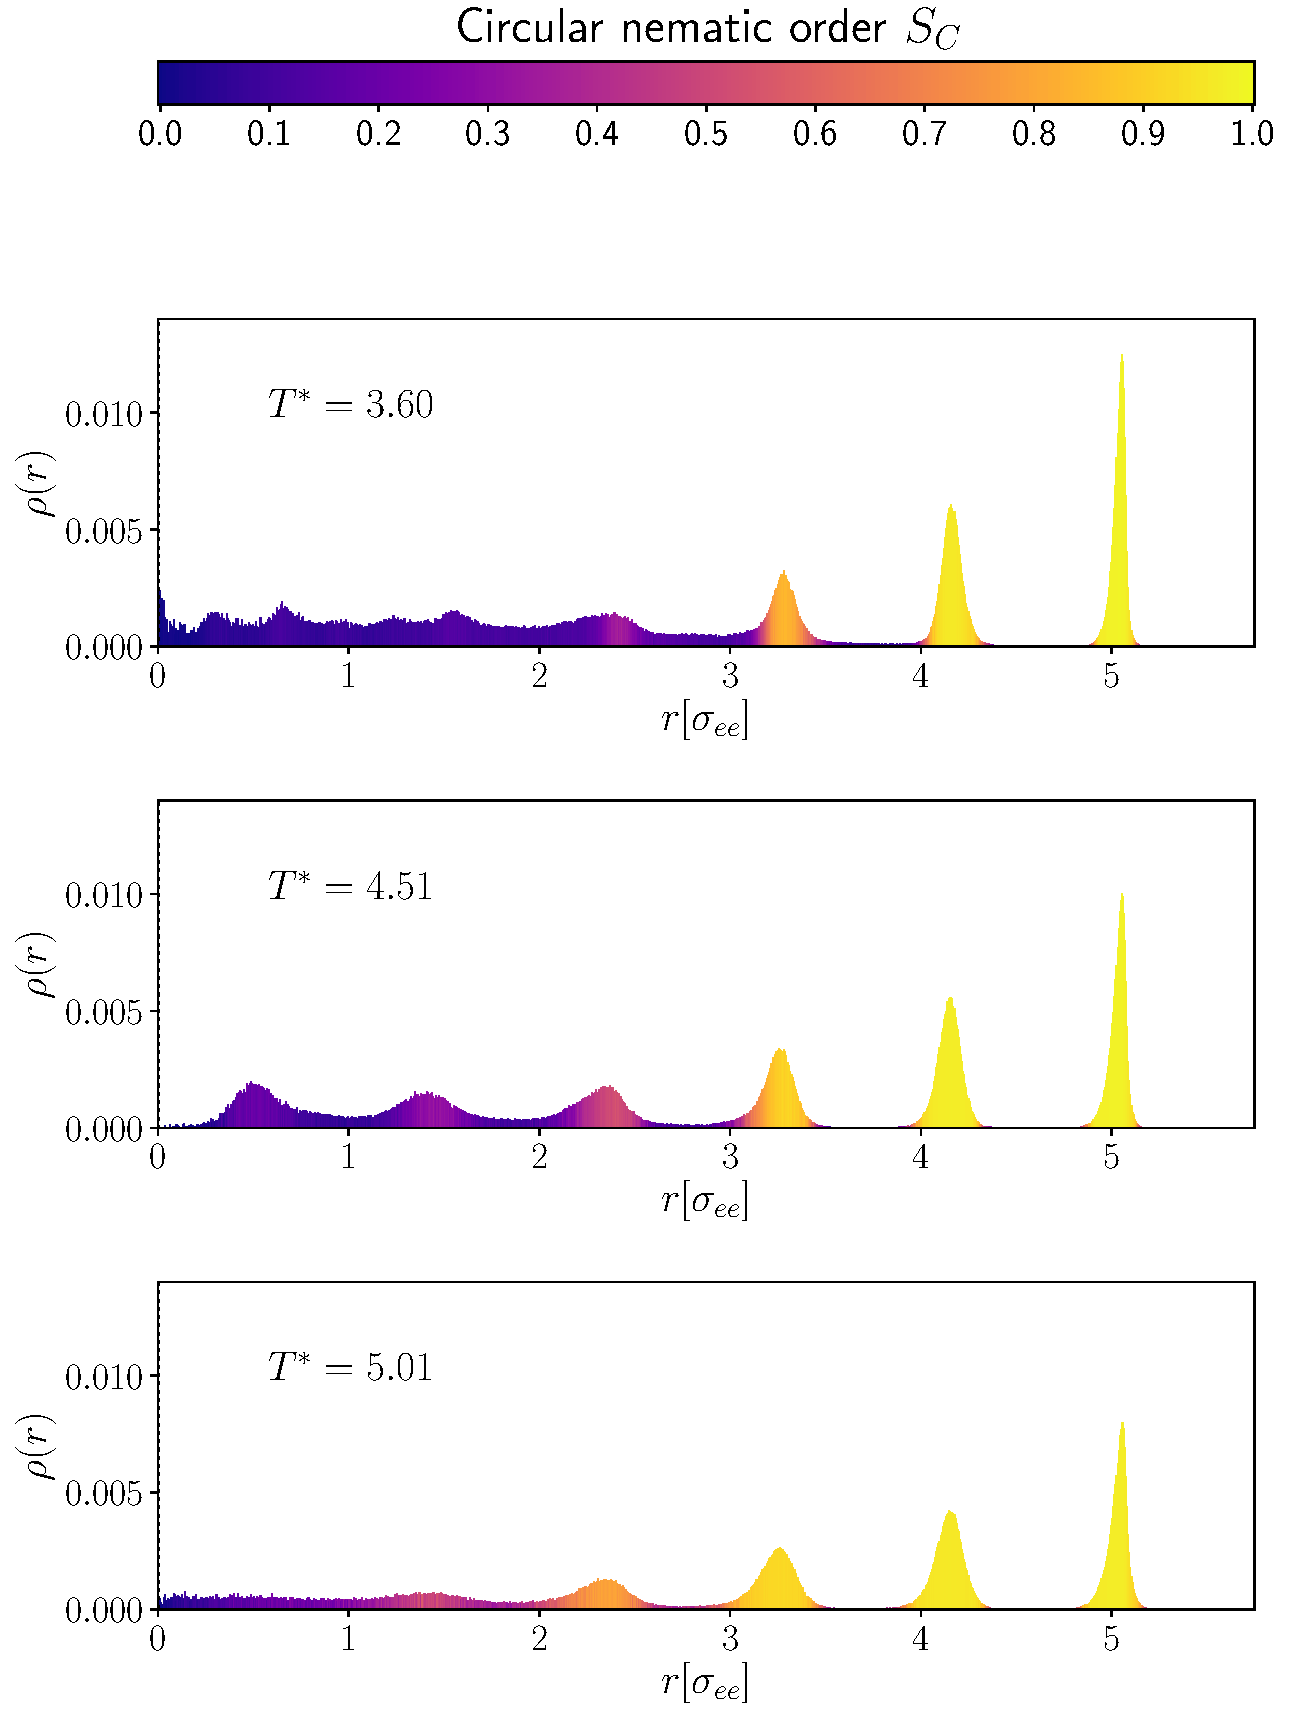
\includegraphics[width=.49\linewidth]{plots/cfo_W8C56_raddensD0.pdf}
 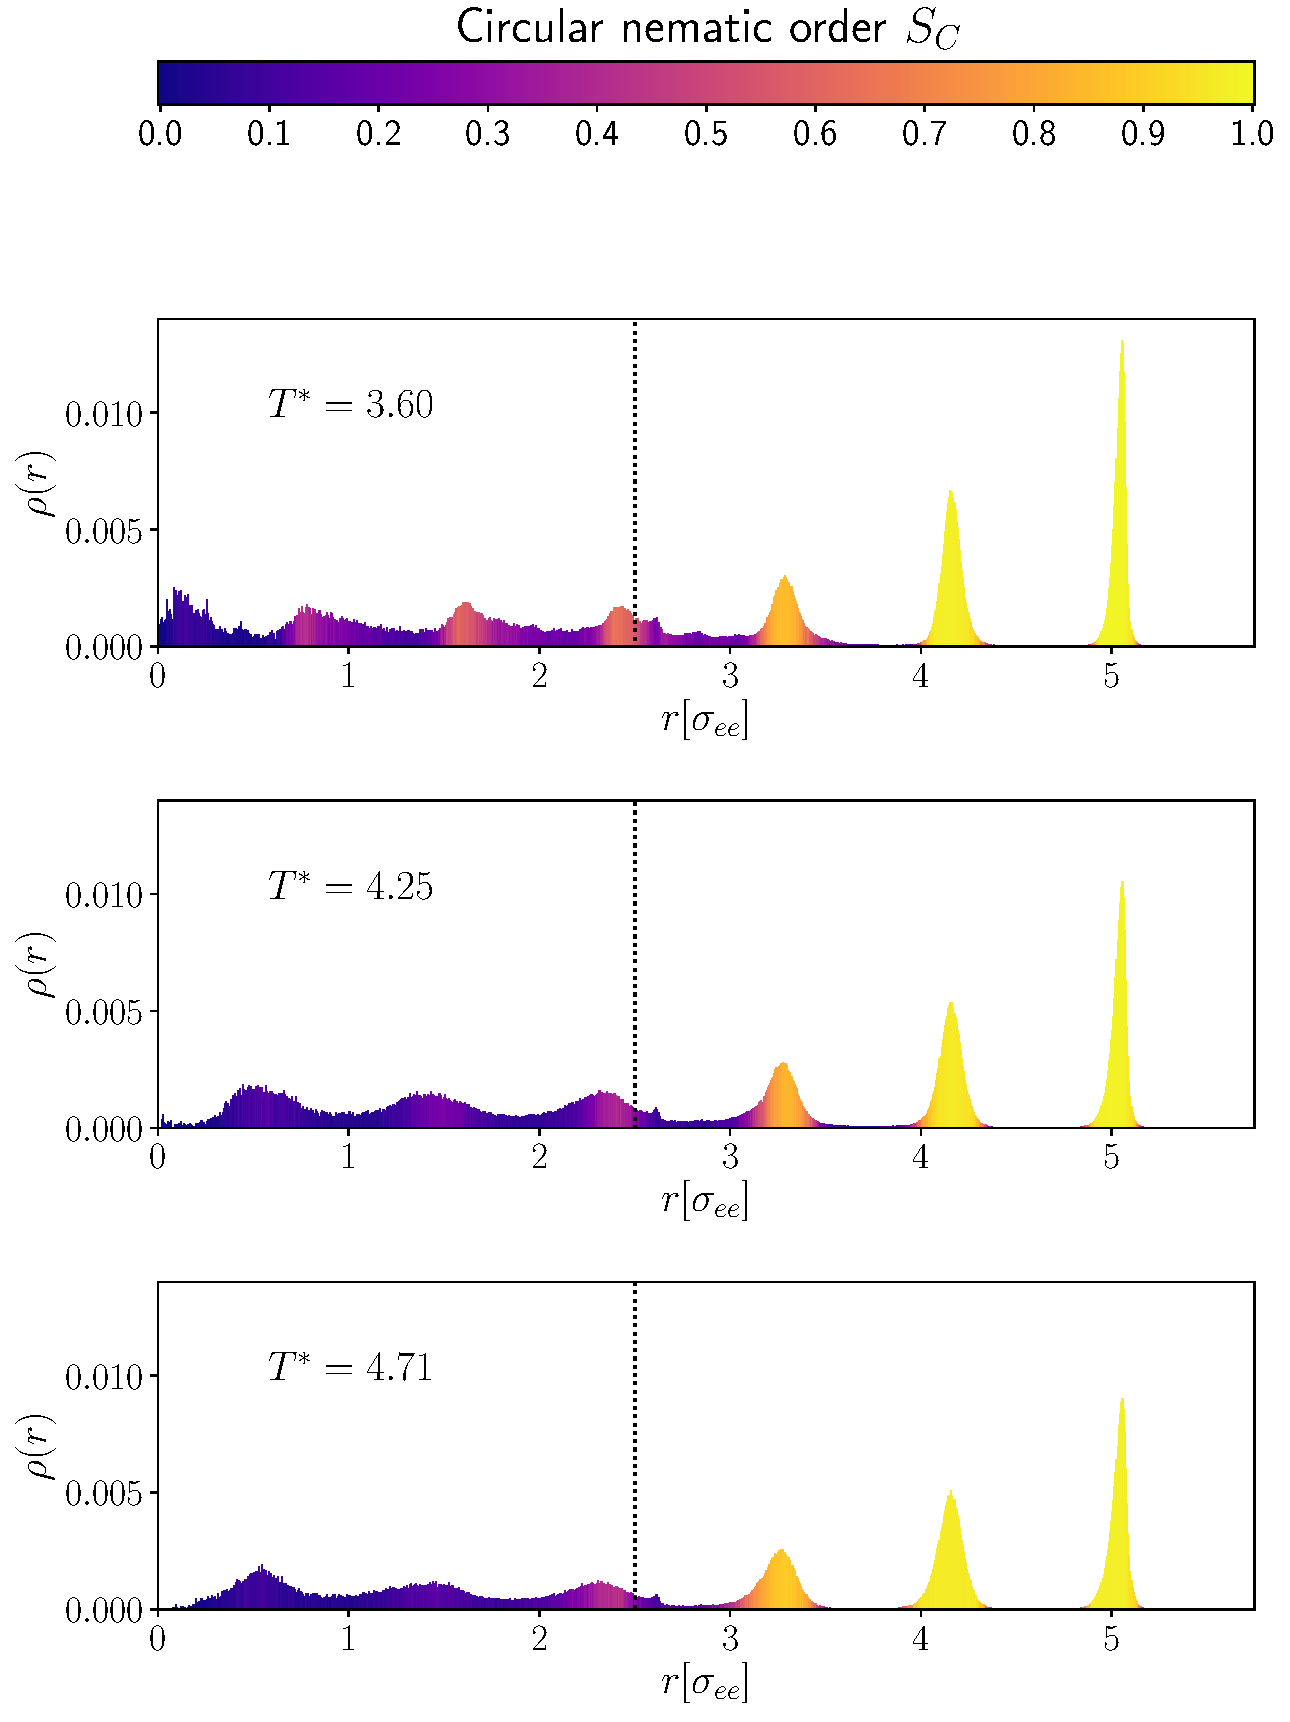
\includegraphics[width=.49\linewidth]{plots/cfo_W8C56_raddensD5.pdf}
\caption{Radial dependence of the local density and circular nematic order at different temperatures for a system without a colloid (left) and a system with a colloid of diameter $D^* = 5$ (right). The vertical dashed line represents the radius of the colloid.}
 \label{fig:bfosnapshots}
\end{figure}

\begin{figure}[H]
 \centering
 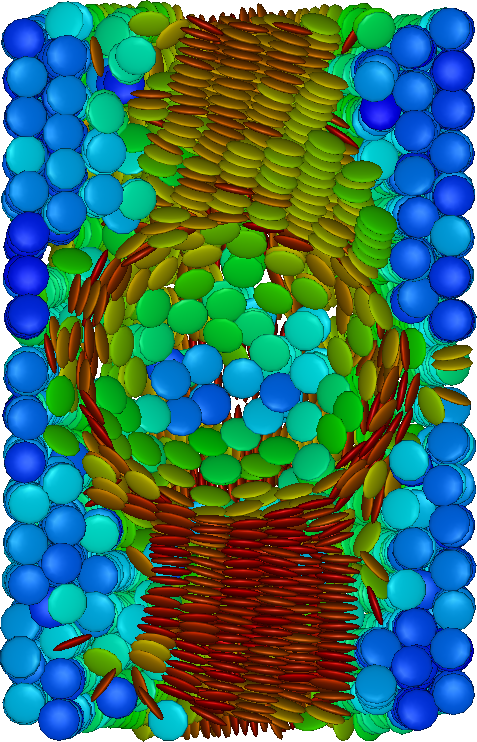
\includegraphics[width=.2\linewidth]{images/cfo_W8C56_D7.png}
\caption{Cross sectional snapshots of the confined discotic liquid crystal system at $P^* = 50$, $T^* = 3.7$ with colloids of diameter $D^*=7 $.}
 \label{fig:cfosnapshots}
\end{figure}



\section{Bulk}
\label{sec:Bulk}
To study the system in bulk we imposed periodic boundary conditions and set a colloidal particle of diameter $D^* \, [\sigma_{ee}]$ in the centre of the system. To try to avoid any small system effects due to the periodic boundary conditions, I had to simulate 10000 particles to offset the size of the colloid, which ranges from $1$ to $10$.\footnote{One possible way to artificially reduce the necessary particle number is to choose a different shape for the simulation box, e.g. a truncated octahedron, that has better sphericity. However, I suspect the box would have to be a regular polyhedron, which may be a disadvantage due to the irregular shape of the particles.} Most effects start appearing only for colloids of diameter $D^* \geq 6$. This takes quite some time (between one and two weeks for one batch of simulations) since the range of temperatures has to be fairly precise so as to avoid any weird effects happening, and the number of performed equilibration steps needs to be increased with the number of particles. therefore the results here are not as complete as I would prefer. In particular the plots of the (global) nematic order parameter in function of the temperature are very noisy, due to the appearance of locally aligned groups of molecules. This could be solved with an even longer run-time, and maybe a few optimizations in the code, which of course would take even longer to run.

\subsection{Edge-On Anchoring}

\begin{figure}[H]
 \centering
 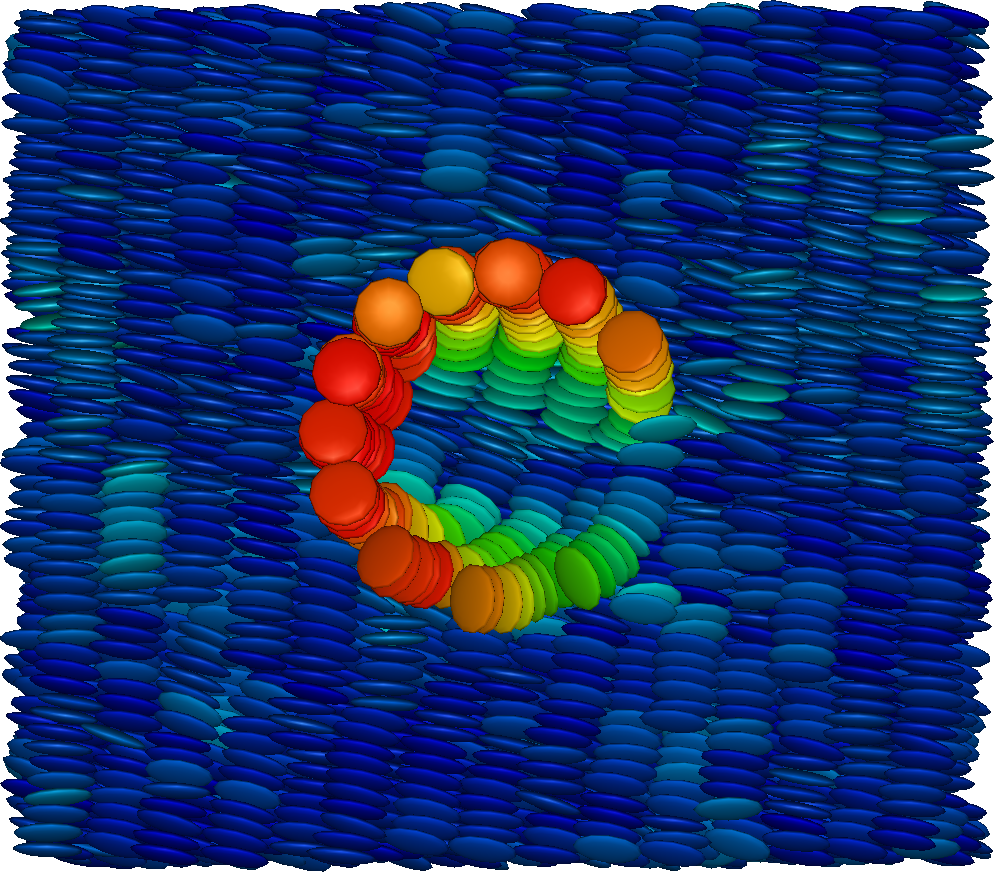
\includegraphics[width=.4\linewidth]{images/beo_C32_D5.png}
 \qquad
 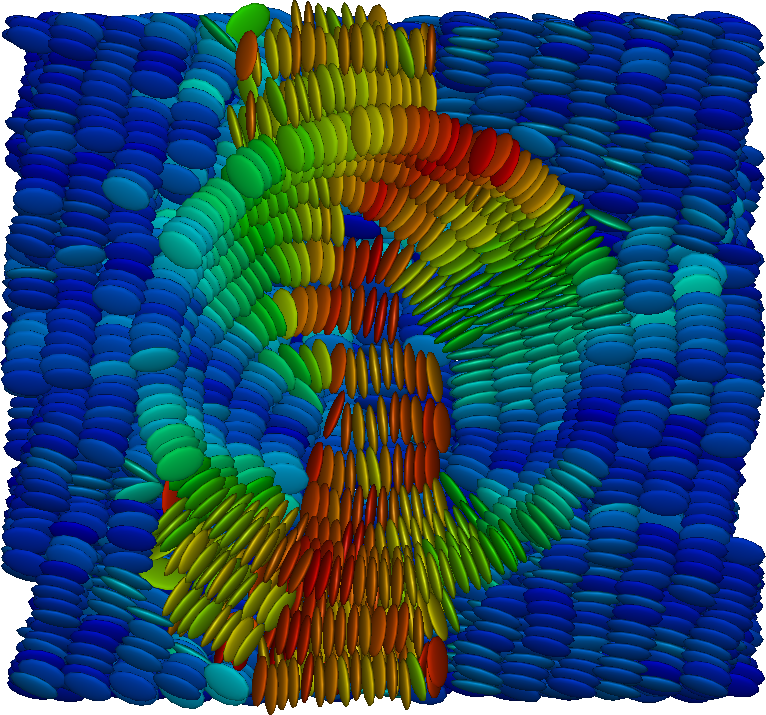
\includegraphics[width=.4\linewidth]{images/beo_C32_D9.png}
\caption{Cross sectional snapshots of the bulk discotic liquid crystal system at $P^* = 50$, $T^* = 4.6$ with colloids of diameter $D^* \in \{5,9\} $.}
 \label{fig:beosnapshots}
\end{figure}


Imposing edge-on anchoring on the colloid we can see in Fig. \ref{fig:beoc32lochex} that the phase transition becomes continuous with the introduction of the colloid. Whereas the bulk system without a colloid displays a first order transition the introduction of the colloid smoothens the transition, giving it a more gradual progression. We can also see that the magnitude og the order parameters in the columnar phase decrease with respect to the colloid size, which is probably due to the layer of discotic particles around the colloid at most temperatures and colloid sizes.
\begin{figure}[H]
    \centering
	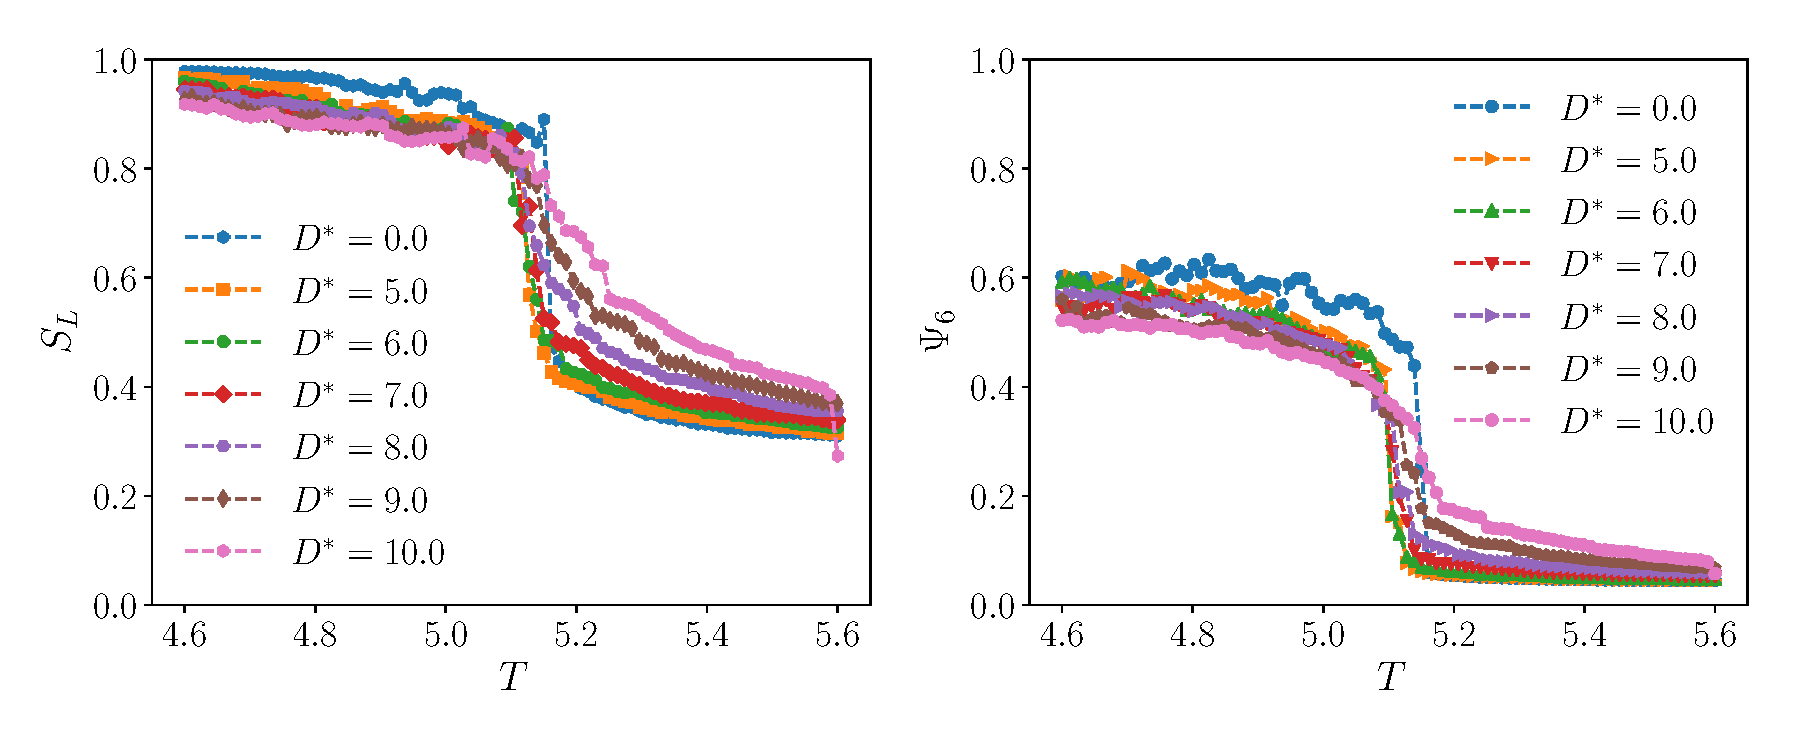
\includegraphics[width=\linewidth]{plots/beo_c32_lochex.pdf}
	\caption{Dependence of the local nematic order parameter and the hexagonal on the temperature for systems in bulk with colloids of different size}
    \label{fig:beoc32lochex}
\end{figure}

If we look at the local radial density in Figure 6 we can see at least one distinct layer of particles near the colloid forming. For the larger colloids we can see the formation of distinct layers that form in the early stages of the columnar phase that start breaking up at lower temperatures due to the tendency of alignment towards the nematic director.
\begin{figure}[H]
    \centering
	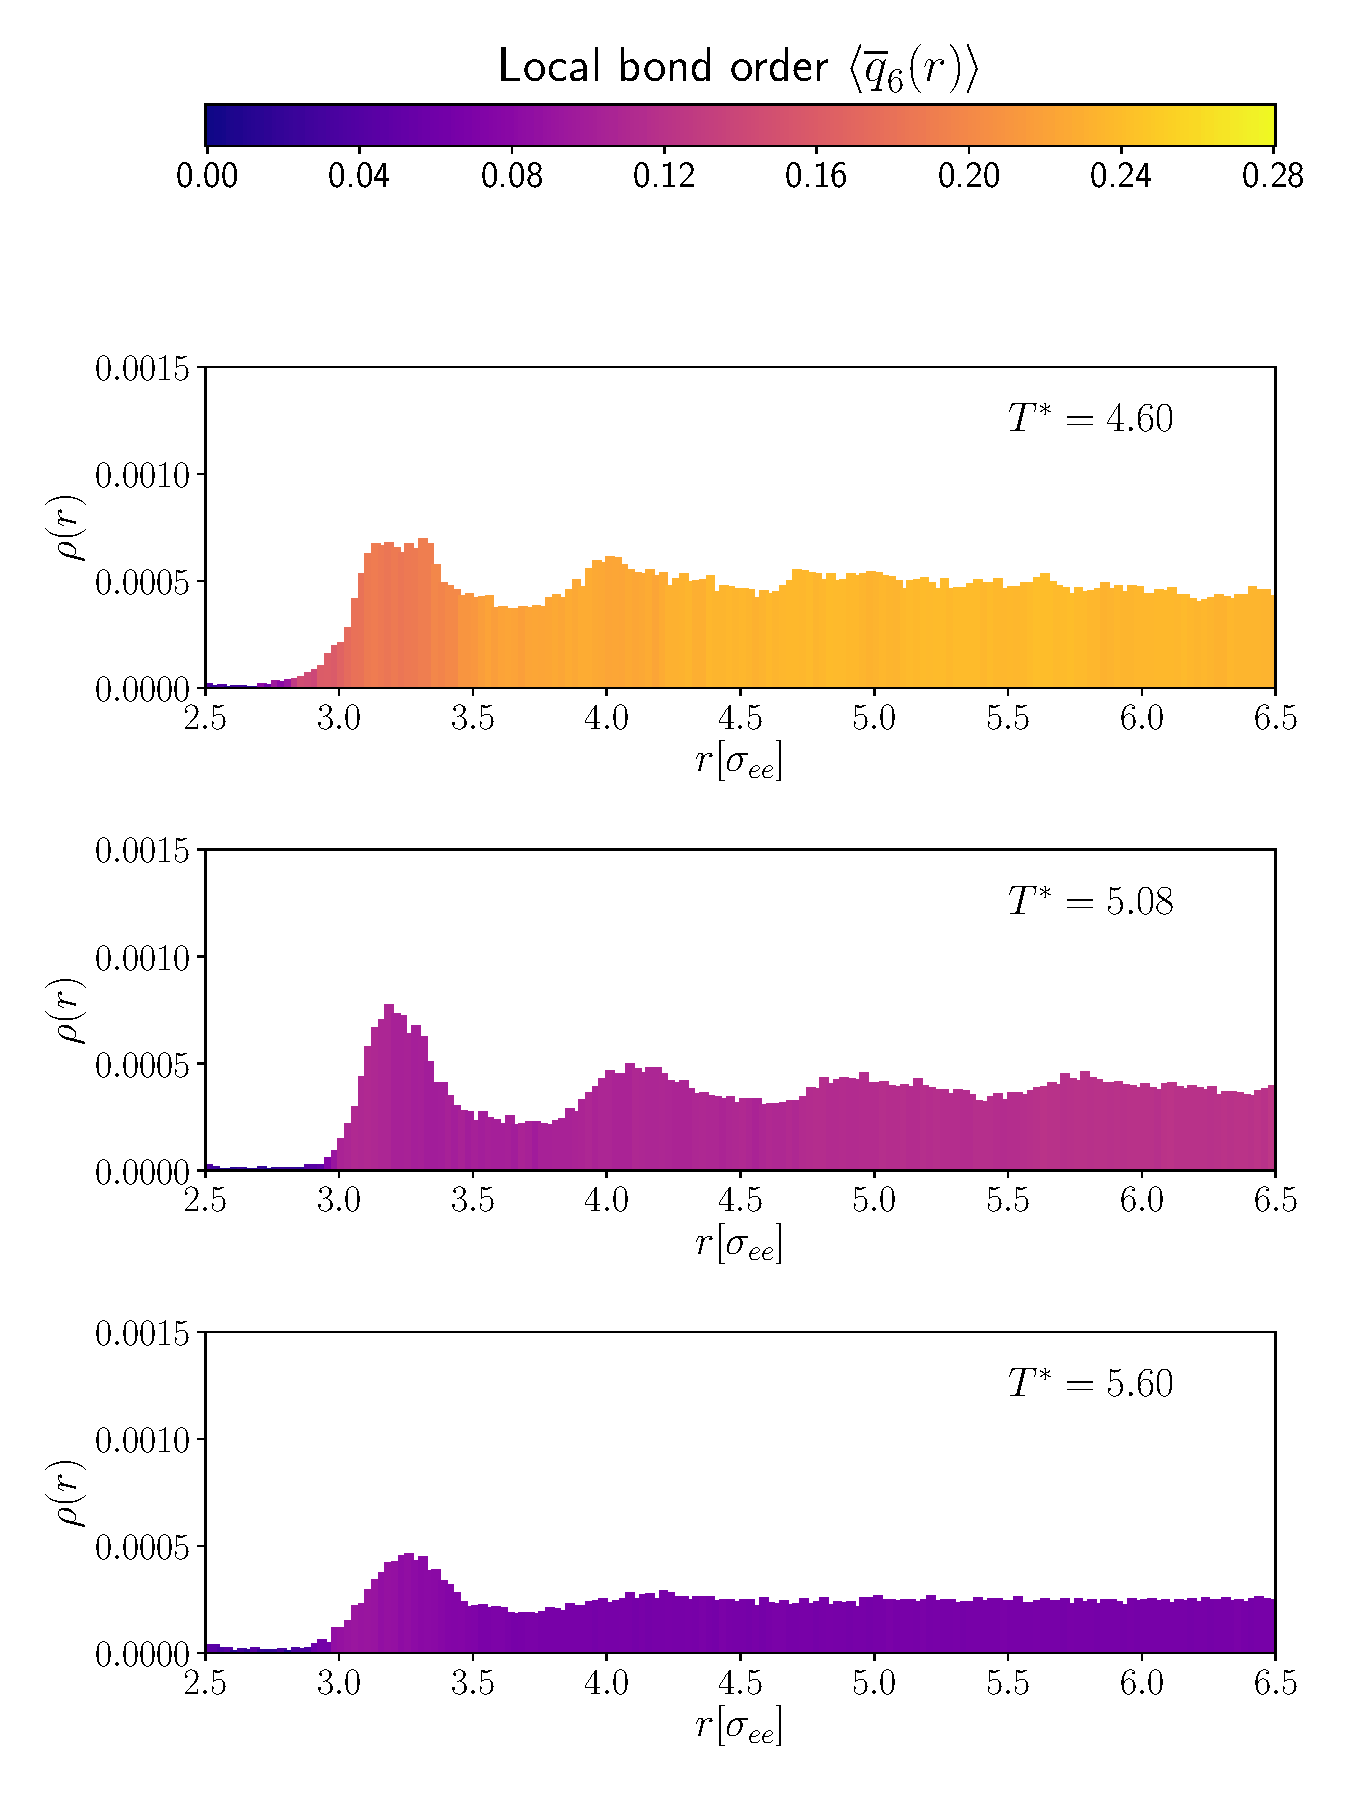
\includegraphics[width=0.49\linewidth]{plots/beo_C32_raddensD5.pdf}
	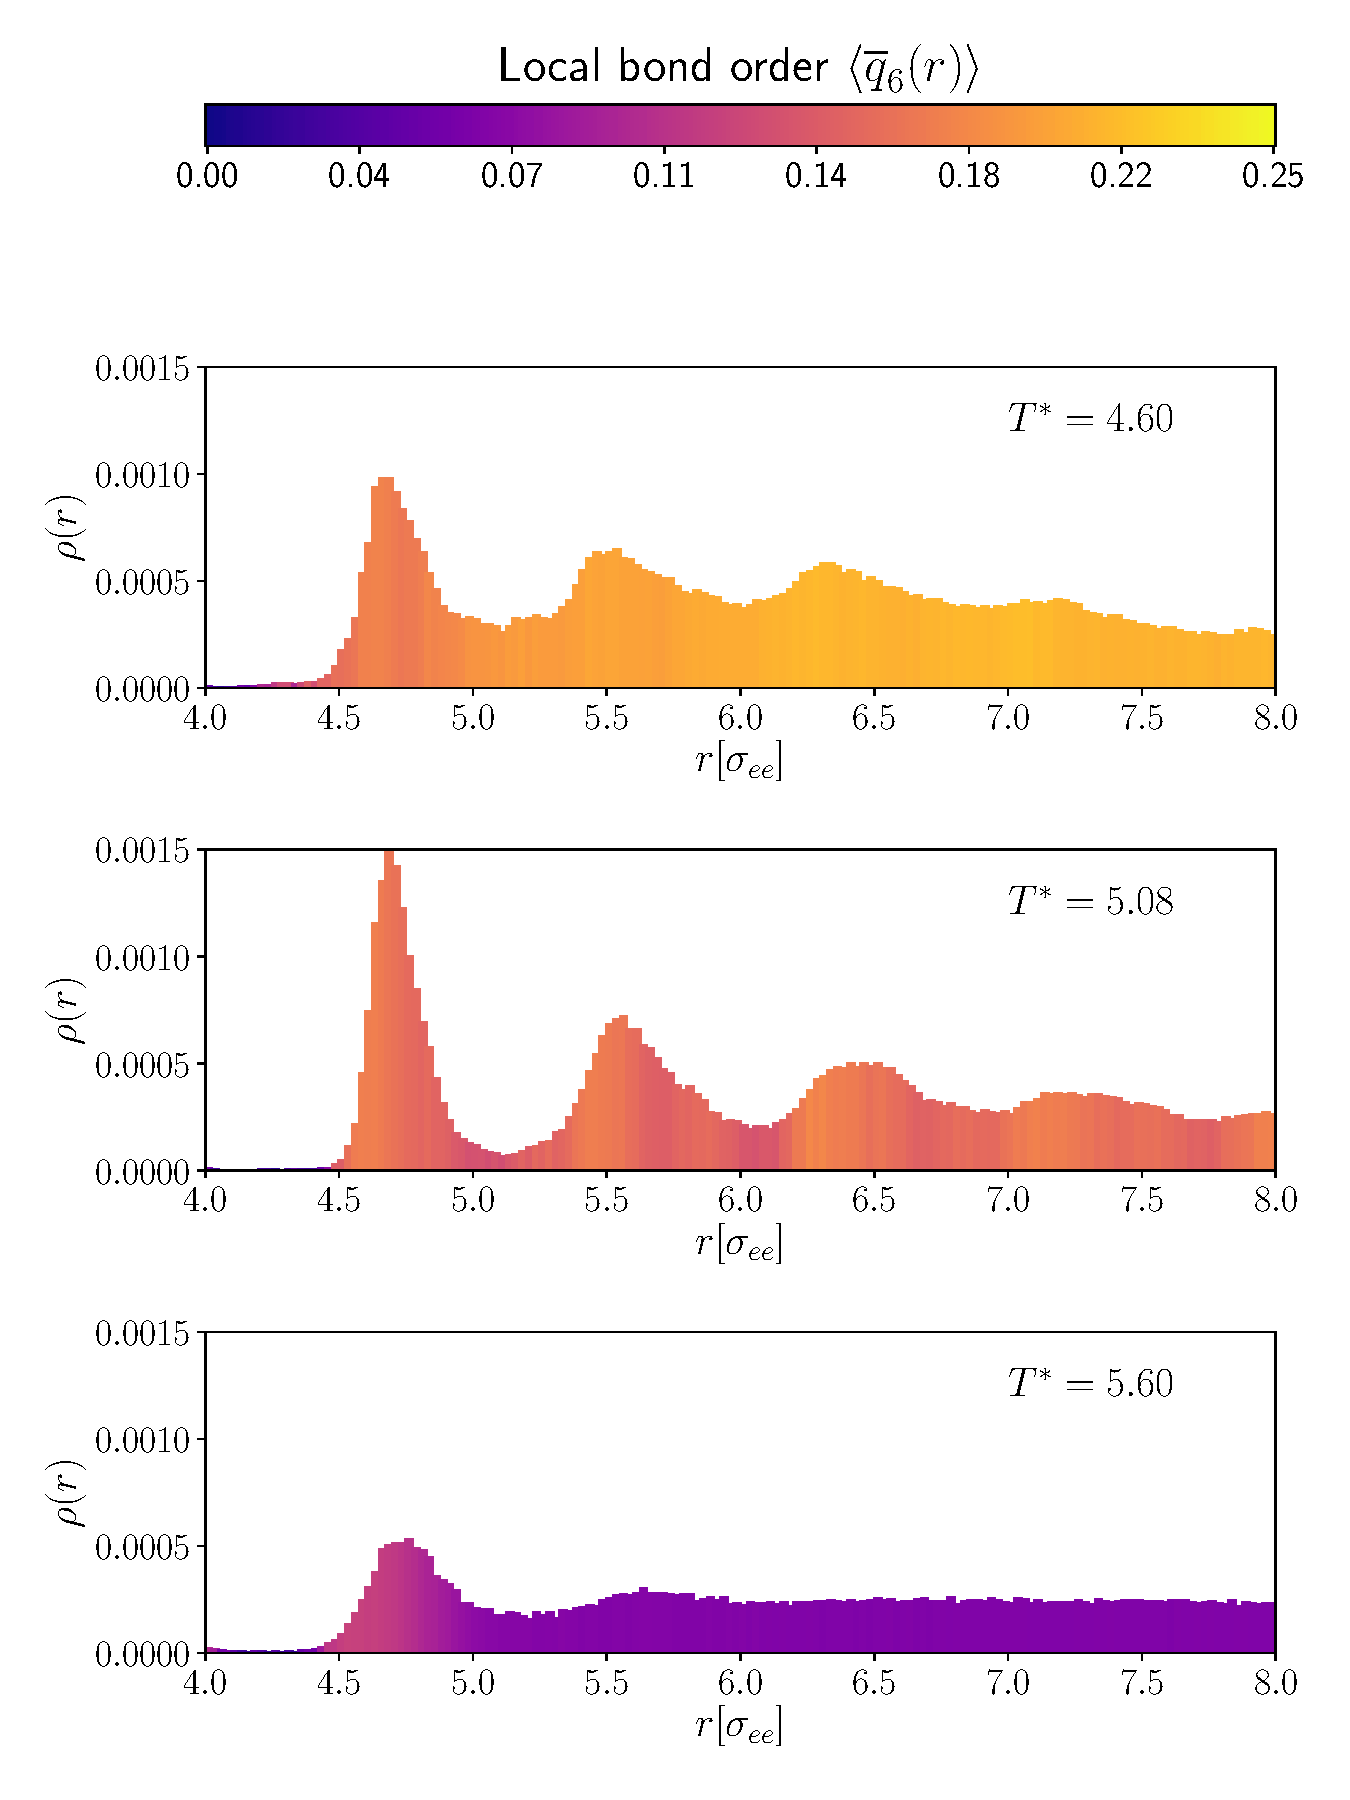
\includegraphics[width=0.49\linewidth]{plots/beo_C32_raddensD8.pdf}
	\caption{Radial dependence of the local density and bond orientational order parameter $ \overline{q}_6$ at different temperatures for a colloid of size $D^* =  5$ (left) and $D^* = 8$ (right)}
    \label{fig:beoc32nemloc}
\end{figure}


\subsection{Face-On Anchoring}


\begin{figure}[H]
 \centering
 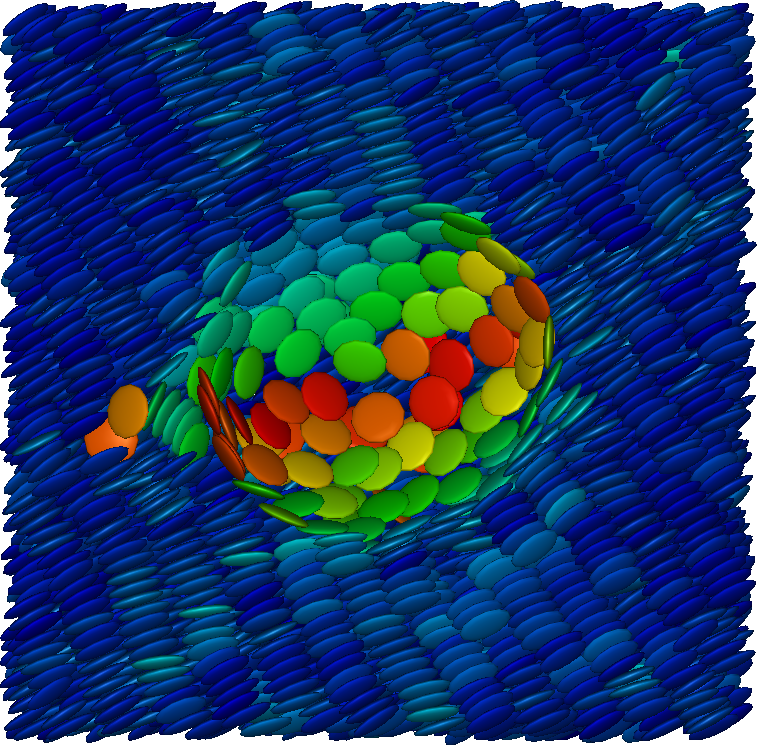
\includegraphics[width=.4\linewidth]{images/bfo_C80_D6.png}
 \qquad
 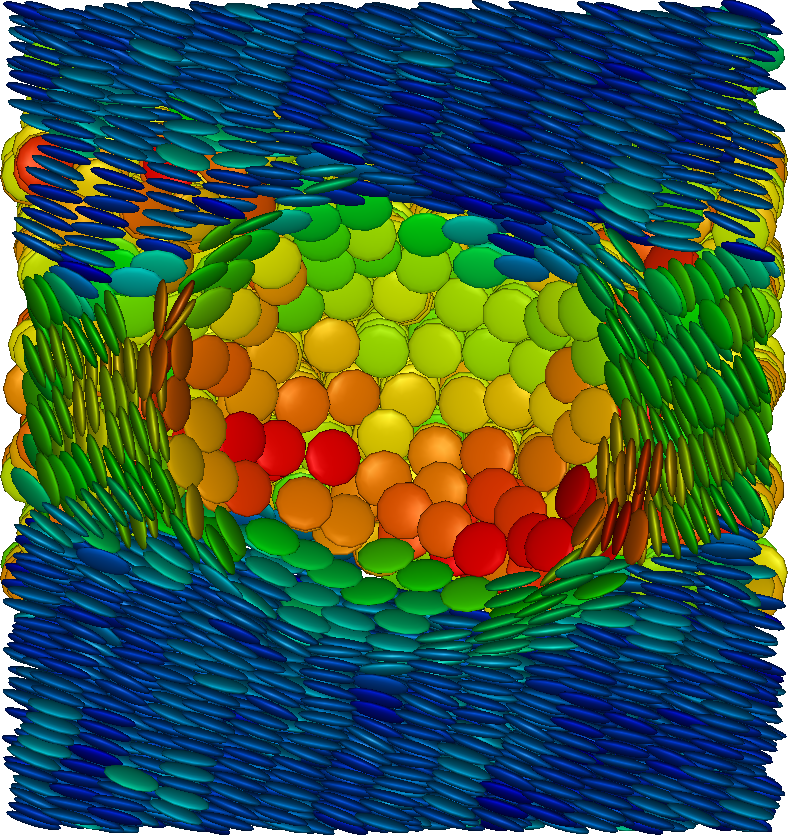
\includegraphics[width=.4\linewidth]{images/bfo_C80_D8.png}
\caption{Cross sectional snapshots of the bulk discotic liquid crystal system at $P^* = 50$, $T^* = 4.5$ with colloids of diameter $D^* \in \{6,8\} $. The colloid potential strength is $\epsilon_{\text{cf}}= 80$. }
 \label{fig:bfosnapshots}
\end{figure}

To study the face-on anchoring I did simulations at different potential strengths, yielding different results.

\subsubsection{Potential strength $\epsilon_{\text{cf}}= 32\epsilon_{\text{ff}}$}
At a potential strength of $\epsilon_{\text{cf}}= 32\epsilon_{\text{cf}}$ there is not much to be seen. The introduction of a colloid does not seem to disturb the system very much, except for a little of the phase transition temperature. Even for the large colloids the nematic order parameter tends towards $1$, which suggests that no layers of molecules form around the colloid. However, due to the slightly higher transition temperature, the colloid probably serves as some sort of nucleating agent. 
\begin{figure}[H]
    \centering
	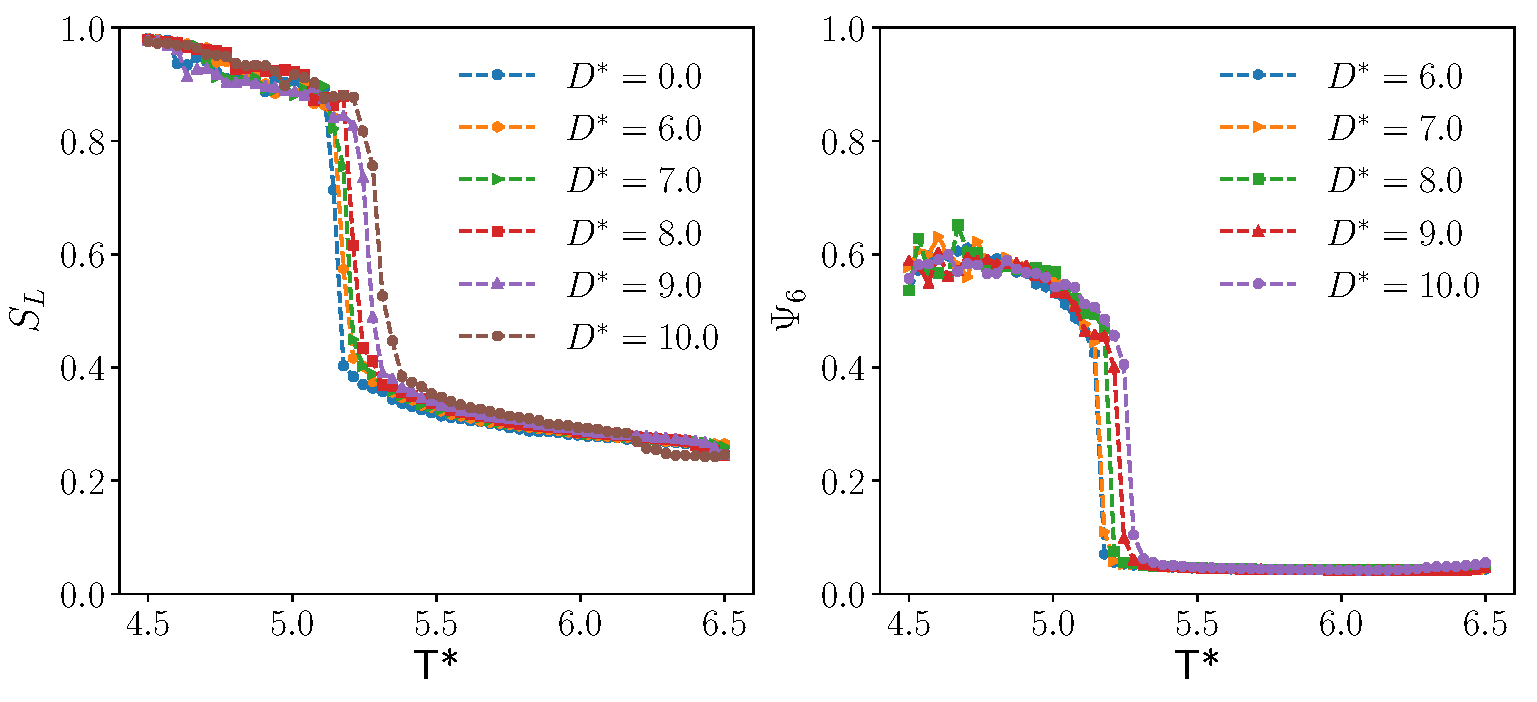
\includegraphics[width=\linewidth]{plots/bfo_C32_nemhex.pdf}
	\caption{Dependence of the local nematic order parameter and the hexagonal on the temperature for systems in bulk with colloids of different size}
    \label{fig:beoc32lochex}
\end{figure}
\begin{figure}[H]
    \centering
	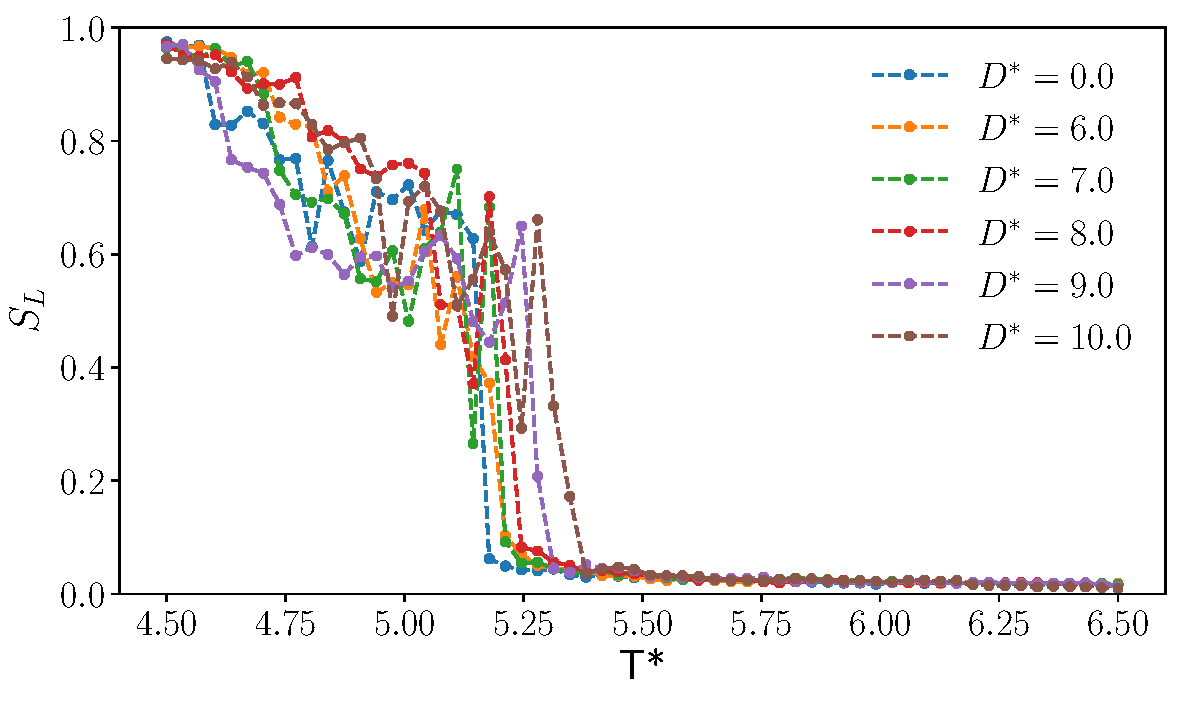
\includegraphics[width=0.7\linewidth]{plots/bfo_C32_nemsca.pdf}
	\caption{Dependence of the nematic order parameter and the hexagonal on the temperature for systems in bulk with colloids of different size}
    \label{fig:beoc32lochex}
\end{figure}


\subsubsection{Potential strength $\epsilon_{\text{cf}}= 80\epsilon_{\text{ff}}$}
Increasing the potential to $\epsilon_{\text{cf}}= 80\epsilon_{\text{ff}}$ we see more substantial results. For smaller colloid sizes ($D^*\in \{6,7,8\}$) we see no difference in the phase transition, whereas with a colloid of diameter $D^*=9.0$ the transition is shifted towards a colder temperature, and with a colloid of diameter $D^*=10.0$ the transition doesn't even appear in the probed temperature range.
\begin{figure}[H]
    \centering
	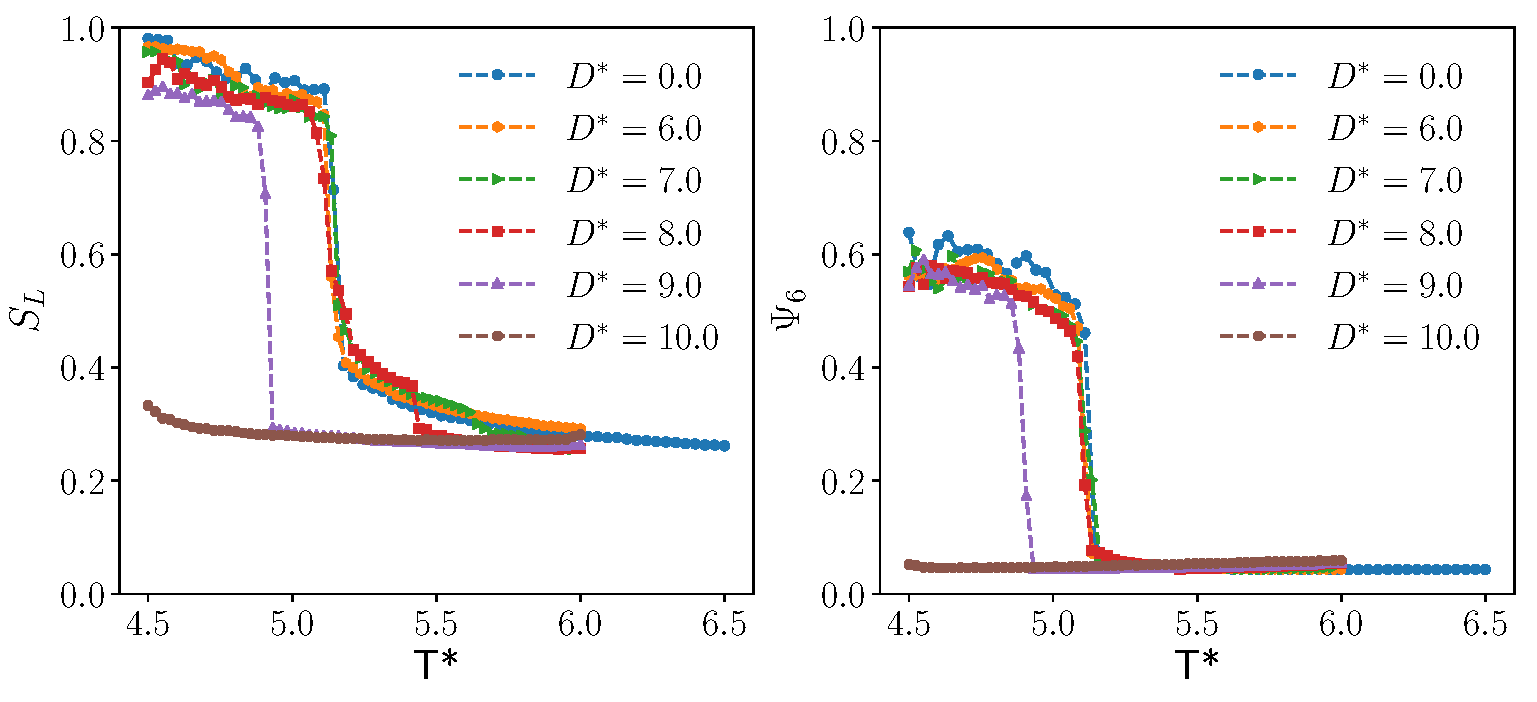
\includegraphics[width=\linewidth]{plots/bfo_C80_nemhex.pdf}
	\caption{Dependence of the local nematic order parameter and the hexagonal on the temperature for systems in bulk with colloids of different size}
    \label{fig:beoc32lochex}
\end{figure}
\begin{figure}[H]
    \centering
	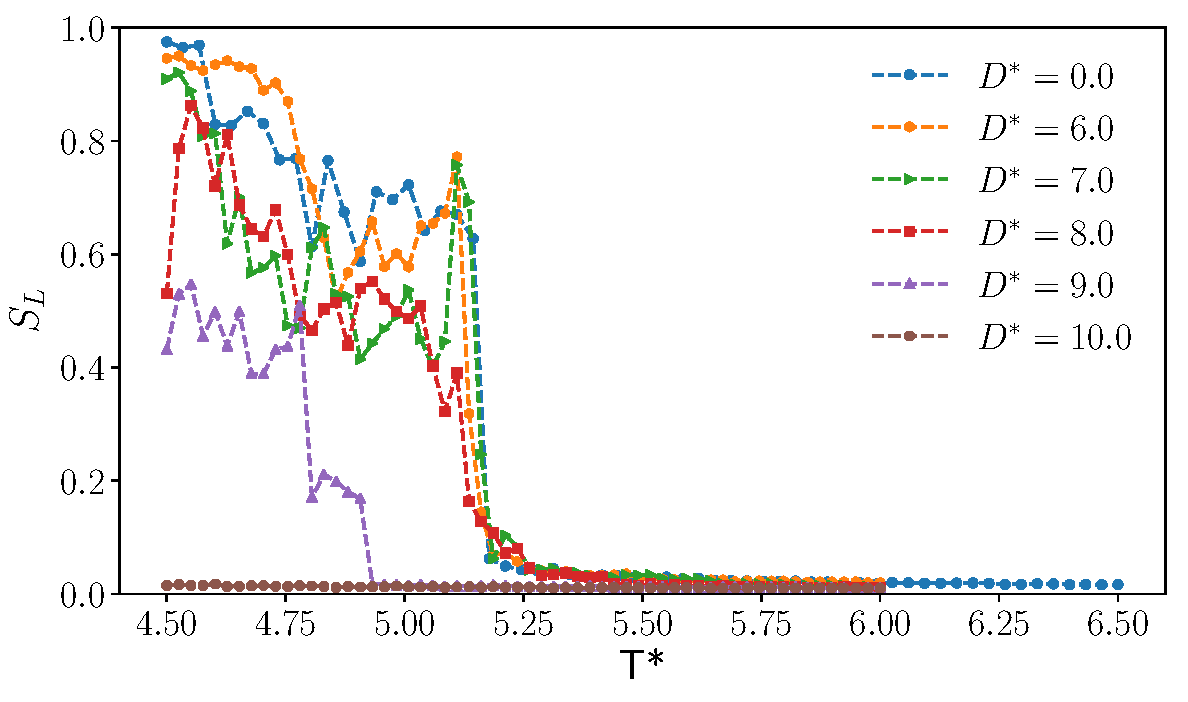
\includegraphics[width=0.7\linewidth]{plots/bfo_C80_nemsca.pdf}
	\caption{Dependence of the nematic order parameter and the hexagonal on the temperature for systems in bulk with colloids of different size}
    \label{fig:beoc32lochex}
\end{figure}

Looking at the the radial density, we can definitely see the formation of layers around the colloid, where the local bond order on these layers is lower than outside, obviously due to the impossibility of formation of radially aligned columns around the colloid.

\begin{figure}[H]
    \centering
	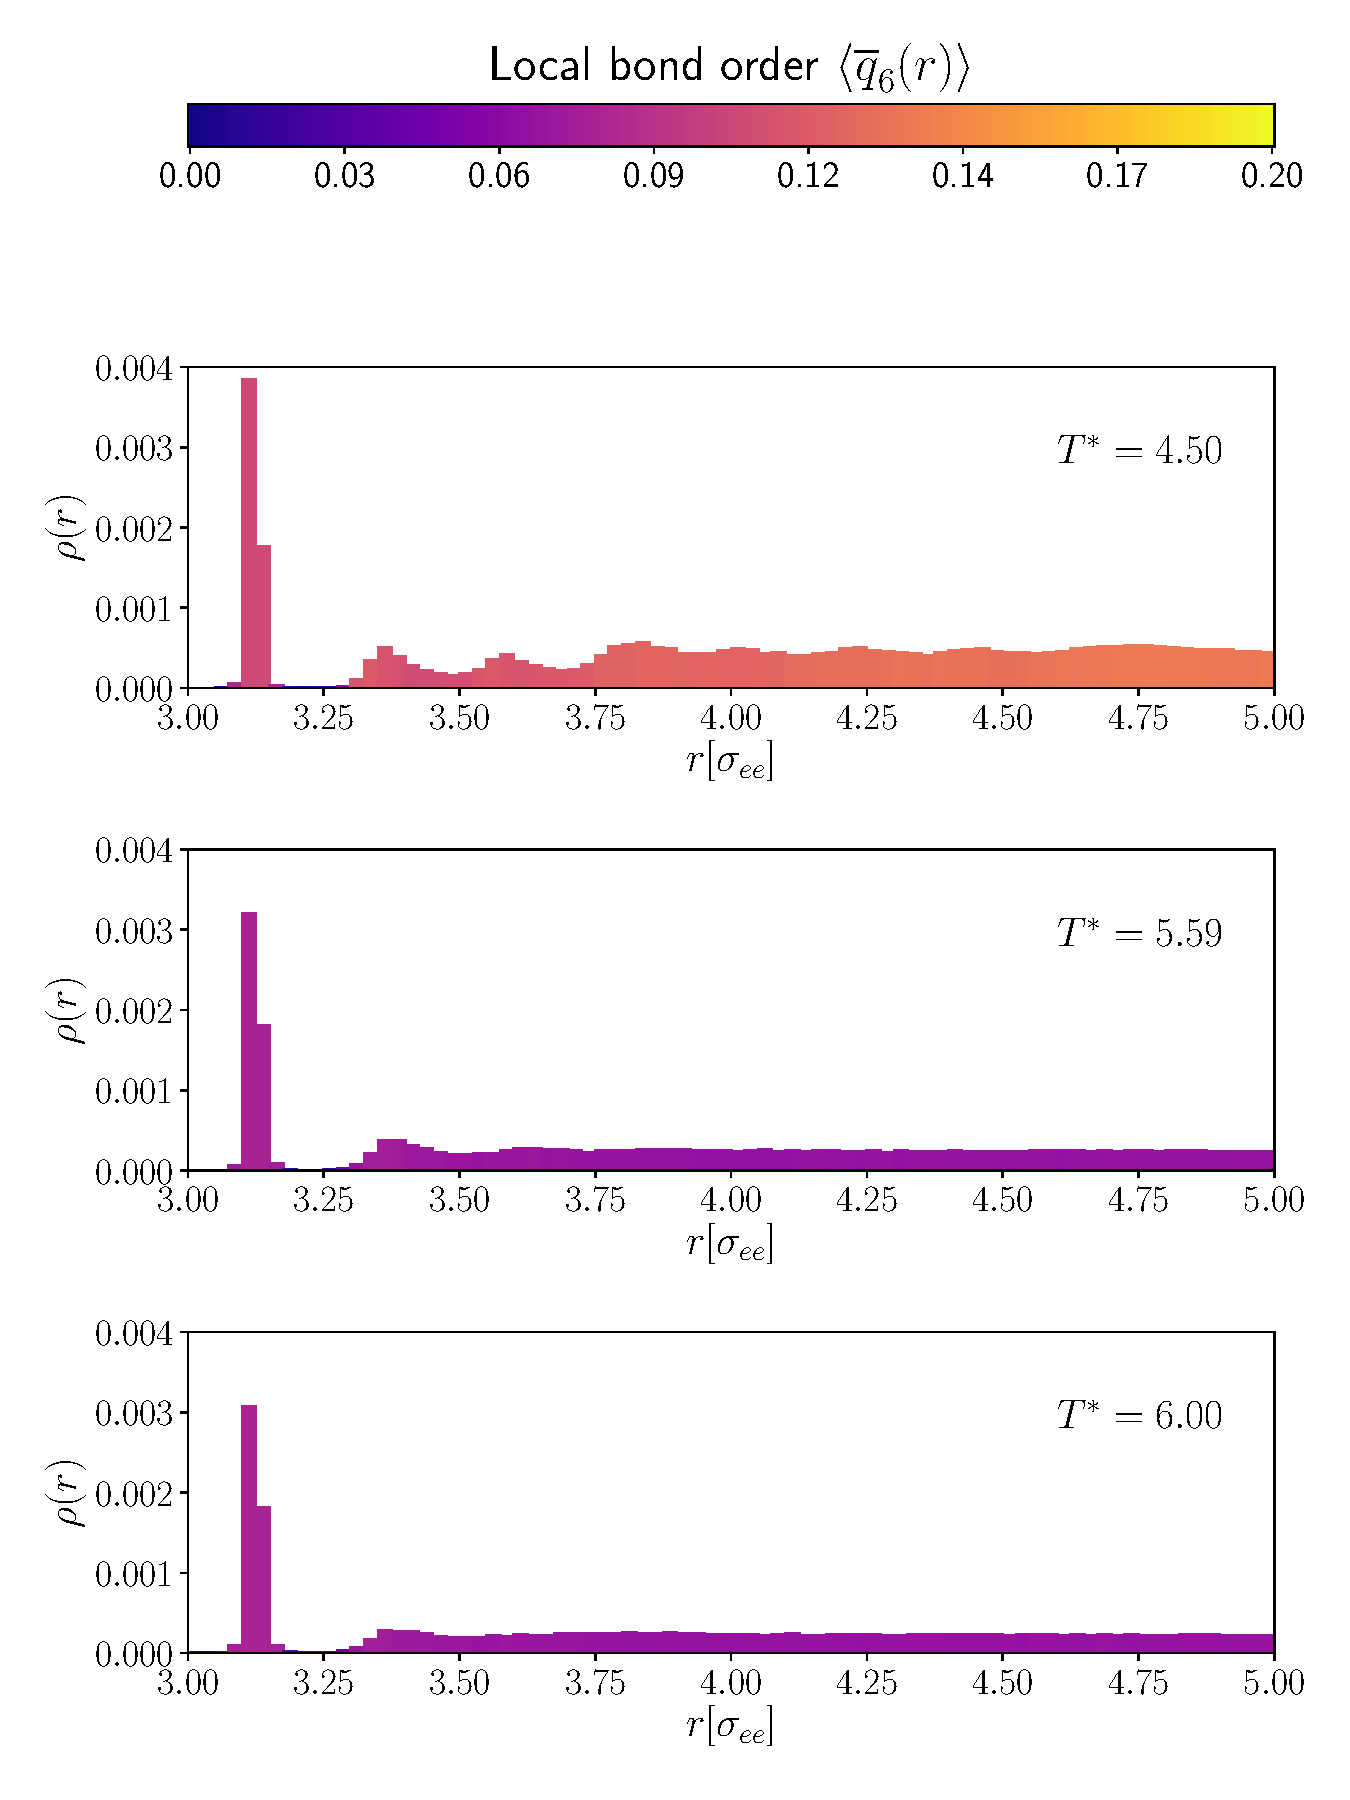
\includegraphics[width=0.49\linewidth]{plots/bfo_C80_raddensD6.pdf}
	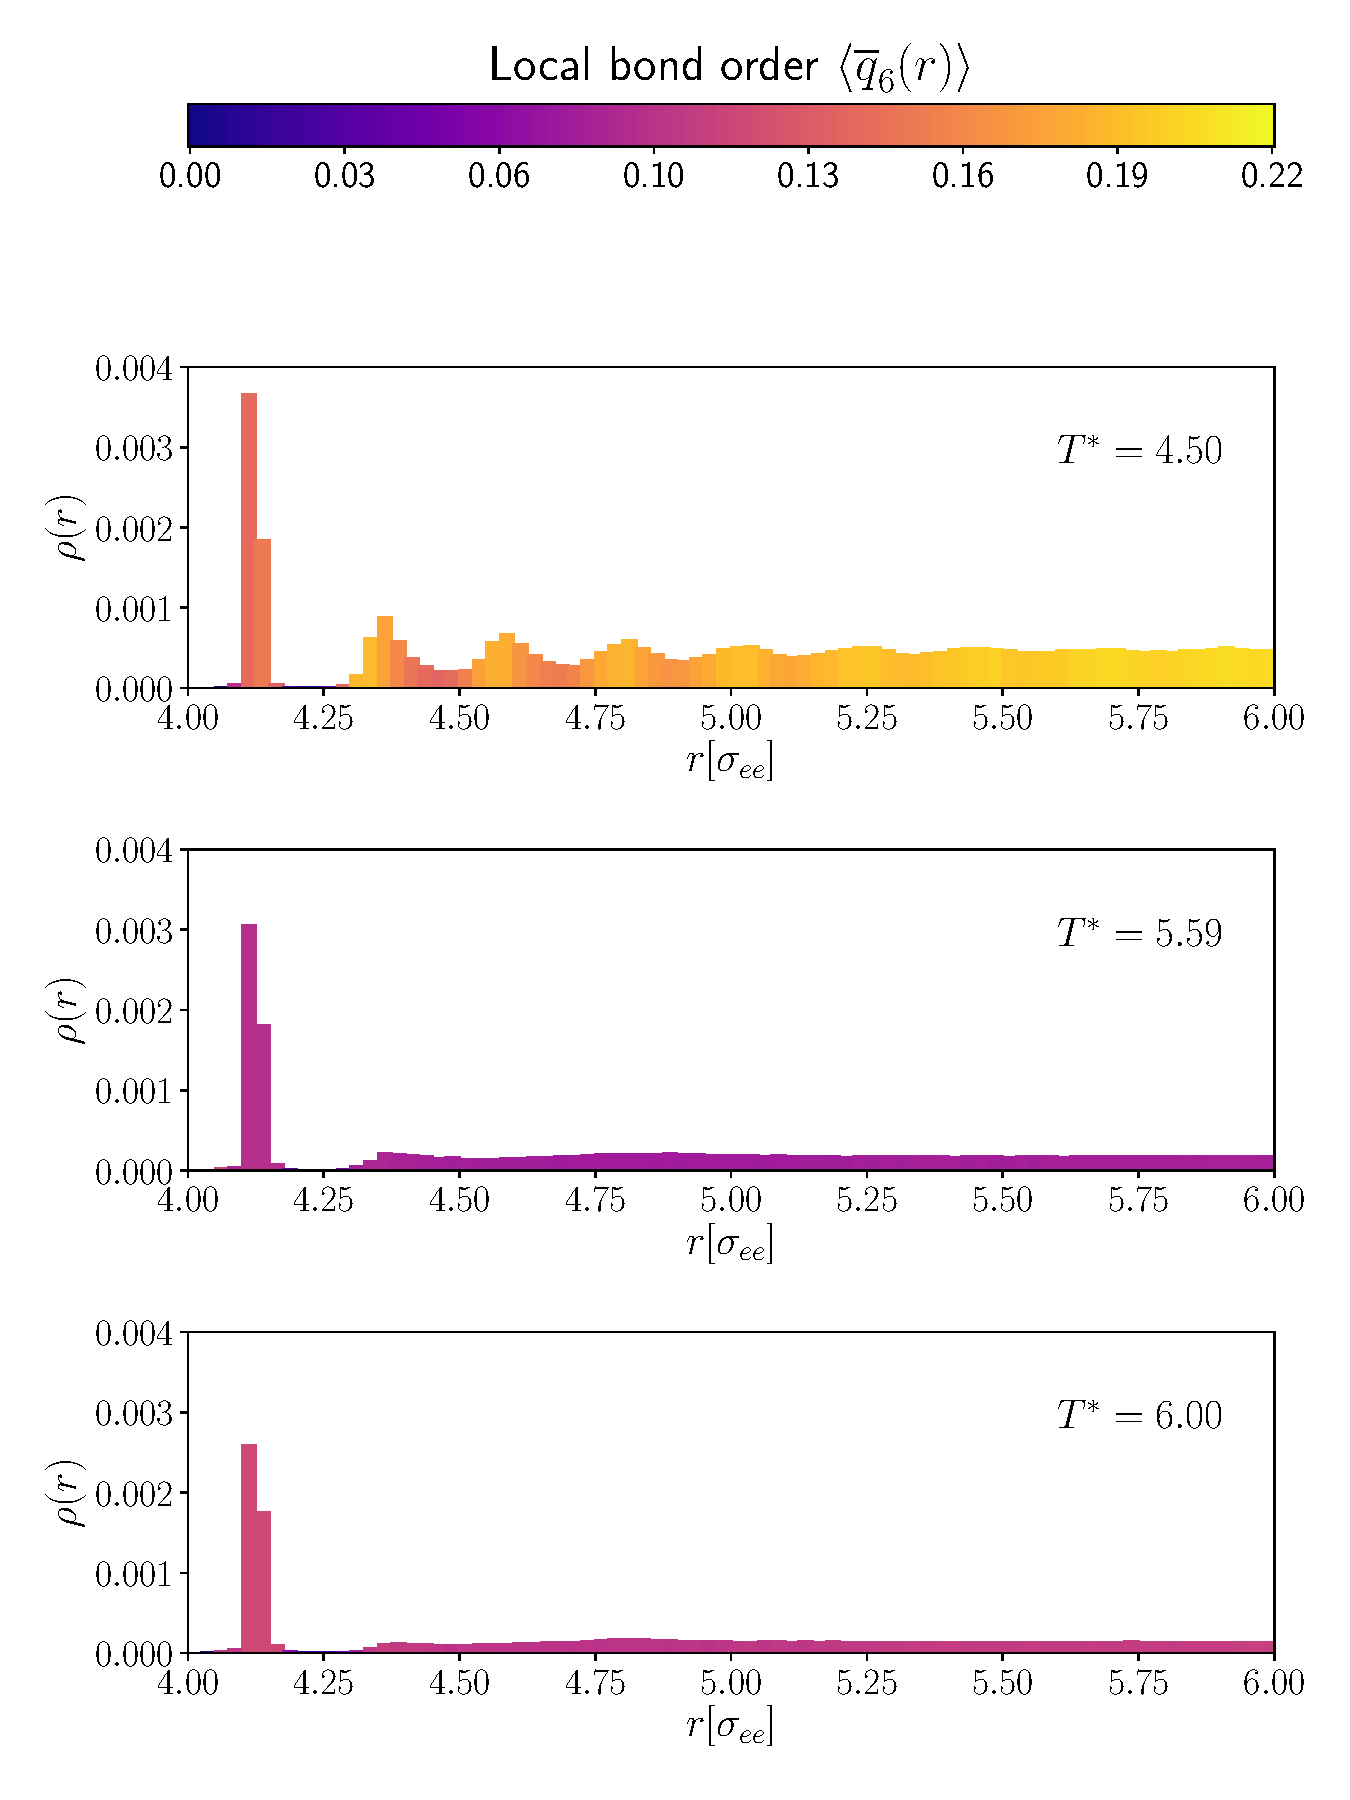
\includegraphics[width=0.49\linewidth]{plots/bfo_C80_raddensD8.pdf}
	\caption{Radial dependence of the local density and bond orientational order parameter $ \overline{q}_6$ at different temperatures for a system with a colloid of size $D^* =  6$ (left) and $D^* = 8$ (right).}
    \label{fig:beoc32nemloc}
\end{figure}


An as of now unfortunately unavoidable factor in these simulations is the small size effect, especially noticeable in Figure \ref{fig:bfosnapshots}. As mentioned in the beginning of this section, increasing the system size may increase the running time by a lot, since the more particles there are, the more steps are required to reach equilibrium. I will try to implement a non-cubic periodic unit cell and see if the improvement is significant.

\chapter{Conclusions}
\vspace{2cm}



%%%%%%%%%%%%%%%%%%%%%%%%%%%%%%%%%%%%%%
%%%%%%%%%%%%%%%%%%%%%%%%%%%%%%%%%%%
\iftrue
%%%%%%%%%%%%%%%%%%%%%%%%%%%%%%%%%%%%%%
%%%%%%%%%%%%%%%%%%%%%%%%%%%%%%%%%%%
\newpage
%\bibliographystyle{unsrt}
\bibliographystyle{joscha_mpi}
\bibliography{citations.bib}
~\newpage
\thispagestyle{empty}
%~\newpage
%%%%%%%%%%%%%%%%%%%%%%%%%%%%%%%%%%%%%%
%%%%%%%%%%%%%%%%%%%%%%%%%%%%%%%%%%%

%\appendix
\setcounter{page}{1}
\pagenumbering{Roman}
\titleformat{\chapter}[hang]
  {\normalfont\huge\bfseries}{}{0pt}{\huge}
\titlespacing*{\chapter}{0pt}{-25pt}{10pt}
%\chapter{Force Derivations}
\chapter*{Appendix}
\addcontentsline{toc}{chapter}{Appendix}
\setcounter{chapter}{1}
\fancyhead[RO]{Appendix}






\fi
\end{document}